\documentclass[a4paper, twoside, symmetric, nobib, nohyper]{tufte-book}
\raggedbottom
% \setcounter{tocdepth}{3}
\setcounter{secnumdepth}{2}
\fancyhead[LE]{Physics simulations, lecture notes}
\fancyhead[RO]{Physics simulations, Chapter \thechapter, section \thesection}
\fancyfoot[LE, RO]{\thepage}

\usepackage{parskip}
\setlength{\parskip}{1.5em}

% Bibliography
\usepackage[
    backend=biber,
    style=authoryear-icomp,
    sortlocale=de_DE,
    natbib=true,
    url=false, 
    doi=true,
    eprint=false
]{biblatex}
\addbibresource{ref/references.bib}

% Math related defs
\usepackage{amsthm, commath, bm, mathtools}

% Cancel terms
\usepackage[thicklines]{cancel}
\renewcommand\CancelColor{\color{xred}}
\newcommand{\cancelcol}[2][xred]{ % This is such a silly solution...
	\renewcommand\CancelColor{\color{#1}}
	\cancel{#2}
	\renewcommand\CancelColor{\color{xred}}
}

% Row- and column-vectors: arguments separated by ";".
% Example: $\vec{a} = \colvec{1;2;3;4}$.
\makeatletter
\newcommand\rcvector[2][\\]{\ensuremath{%
  \global\def\rc@delim{#1}%
    \negthinspace\begin{bmatrix}
      \rc@vector #2;\relax\noexpand\@eolst%
    \end{bmatrix}}}
\def\rc@vector #1;#2\@eolst{%
  \ifx\relax#2\relax
    #1
  \else
    #1\rc@delim
    \rc@vector #2\@eolst%
  \fi}
\makeatother
\newcommand{\colvec}{\rcvector}
\newcommand{\rowvec}[1]{\rcvector[,\;]{#1}}
\newcommand{\GenericRowVec}[2][n]{\rowvec{#2_{1};#2_{2};\dots;#2_{#1}}}
\newcommand{\GenericColVec}[2][n]{\colvec{#2^{1};#2^{2};\vdots;#2^{#1}}}

% Easier space-notation
\newcommand{\Rs}[1][]{\mathbb{R}^{#1}}
\newcommand{\Cs}[1][]{\mathbb{C}^{#1}}

% Better imaginary unit and natural base notation (to separate from variables)
\newcommand{\iu}{\mathrm{i}\mkern1mu}
\newcommand{\eu}{\mathrm{e}}
\newcommand{\Eu}[1]{\mathrm{e}^{#1}}
\newcommand{\EX}[1]{\exp\left(#1\right)}

% Norms and the like
\renewcommand{\norm}[1]{\left\| #1 \right\|}
\newcommand{\vnorm}[1]{\left\| \vec{#1} \right\|}

% Physics stuff
\usepackage{physics}
\usepackage[separate-uncertainty=true]{siunitx}
\renewcommand{\SI}[3][]{\mbox{$\num[#1]{#2}\,\left[\si{#3}\right]$}}
\newcommand{\SIe}[1]{\SI{}{#1}}

% Graphics
\usepackage{tikz}
\usetikzlibrary{calc, positioning, arrows.meta, decorations.pathmorphing, decorations.text, decorations.pathreplacing, patterns}
\tikzset{
  vector/.style = {#1, ultra thick, -stealth, cap=round},
  springcoil/.style={thick, decoration={aspect=0.3, segment length=3mm, amplitude=3mm, coil}, decorate},
}
\usepackage{pgfplots}
\usepgfplotslibrary{colormaps}
\pgfplotsset{
	compat=1.16,
	every axis/.append style={font=\small},
	function/.style n args={1}{line width=1.5pt, color=#1},
	graph2d/.style={
		trig format plots=rad,
		axis x line=middle,
		axis y line=middle,
		every axis x label/.style={
			at={(ticklabel* cs:1.01)},
			anchor=west,
		},
		every axis y label/.style={
			at={(ticklabel* cs:1.01)},
			anchor=south,
		},
		axis line style={stealth-stealth, thick},
		label style={font=\large},
		xlabel=$x$,
		ylabel=$y$,
		tick label style={font=\small},
		samples=200,
		grid=both,
		grid style={line width=.1pt, draw=gray!20},
		major grid style={line width=.2pt,draw=gray!50},
		minor tick num=4,
	},
}

% Colors
\definecolor{xred}{HTML}{BD4242}
\definecolor{xblue}{HTML}{4268BD}
\definecolor{xgreen}{HTML}{52B256}
\definecolor{xpurple}{HTML}{7F52B2}
\definecolor{xorange}{HTML}{FD9337}
\definecolor{xdotted}{HTML}{999999}
\definecolor{xgray}{HTML}{777777}
\definecolor{xcyan}{HTML}{80F5DC}
\definecolor{xpink}{HTML}{F690EA}
\definecolor{xgrayblue}{HTML}{49B095}
\definecolor{xgraycyan}{HTML}{5AA1B9}

\colorlet{xdarkred}{xred!50!black}
\colorlet{xdarkblue}{xblue!50!black}
\colorlet{xdarkgreen}{xgreen!50!black}
\colorlet{xdarkpurple}{xpurple!50!black}
\colorlet{xdarkorange}{xorange!50!black}

% \usepackage{enumitem}

% Font-related stuff
\usepackage{fontawesome}

% Fancy environments
\usepackage[most]{tcolorbox}
\newenvironment{descitemize}
{\begin{description}[leftmargin=*, before=\let\makelabel\descitemlabel]}
{\end{description}}
\newcommand{\descitemlabel}[1]{\textbullet\ \textbf{#1}:}

\usepackage[most]{tcolorbox}

\tikzset{
	second box/.style={
		anchor=east,
		text=white,
		% rounded corners,
		fill=#1,
		xshift=-4mm,
	},
}
\tikzset{tcbreak/.style = {fill=white, thick, draw=#1, text=#1, font=\bfseries}}
\tcbset{
	common/.style n args={2}{
		colframe={#1},
		colback={#1!5},
		colbacktitle={#1},
		lower separated=false,
		coltitle=white,
		boxrule=1pt,
		fonttitle=\bfseries,
		enhanced,
		breakable,
		top=8pt,
		sharp corners,
		before skip=1em,
		after skip=2em,
		attach boxed title to top left={
			yshift=-0.25cm,
			xshift=0.38cm,
		},
		boxed title style={
			boxrule=0pt,
			colframe=white,
			arc=0pt,
			outer arc=0pt,
		},
		separator sign={~~},
		% -- overlays based on the following TeX SE answer: https://tex.stackexchange.com/a/545324/162087
		overlay unbroken={
			\node[text=white, align=right, fill=#1, xshift=-4mm, minimum height=6mm, anchor=east] at (frame.south east) {#2};
		},
		overlay first={
			\draw[thick, #1, decoration={coil, amplitude=0.5mm}, decorate]
				(frame.south west) -- (frame.south east);
			\path[font=\small\itshape] (frame.south) node [tcbreak={#1}] (cont) {continues in the next page \faHandORight};
		},
		overlay middle={%
			% upper break
			\draw[thick, #1, decoration={coil, amplitude=0.5mm}, decorate]
				(frame.north west) -- (frame.north east);
			\path[font=\small\itshape] (frame.north) node [tcbreak={#1}] (cont) {\faHandORight continues from the previous page};

			% lower break
			\draw[thick, #1, decoration={coil, amplitude=0.5mm}, decorate]
				(frame.south west) -- (frame.south east);
			\path[font=\small\itshape] (frame.south) node [tcbreak={#1}] (cont) {continues in the next page \faHandORight};
		},
		overlay last={
			\node[text=white, align=right, fill=#1, xshift=-4mm, minimum height=6mm, anchor=east] at (frame.south east) {#2};
			\draw[thick, #1, decoration={coil, amplitude=0.5mm}, decorate]
				(frame.north west) -- (frame.north east);
			\path[font=\small\itshape] (frame.north) node [tcbreak={#1}] (cont) {\faHandORight continues from the previous page};
		}
	},
	defstyle/.style={
		common={xpurple}{$\bm{\pi}$},
	},
	theoremstyle/.style={
		common={xgraycyan}{$\multimapdotbothA$},
	},
	lemmastyle/.style={
		common={xgrayblue}{$\multimap$},
	},
	proofstyle/.style={
		common={xgreen}{\textbf{QED}},
	},
	examplestyle/.style={
		common={xblue}{\faStar},
	},
	notestyle/.style={
		common={xred}{\textbf{!}},
	},
	challengestyle/.style={
		common={xgreen}{\textbf{?}},
	},
	quotestyle/.style={
		common={gray}{\textbf{"}},
	},
}

\newtcbtheorem[auto counter, number within=chapter]{definition}{Definition}{defstyle}{def}
\newtcbtheorem[auto counter, number within=chapter]{theorem}{Theorem}{theoremstyle}{theorem}
\newtcbtheorem[auto counter, number within=chapter]{lemma}{Lemma}{lemmastyle}{lemma}
% \newtcbtheorem[auto counter, number within=chapter]{proof}{Proof}{proofstyle}{proof}
\newtcbtheorem[auto counter, number within=chapter]{example}{Example}{examplestyle}{example}
\newtcbtheorem[auto counter, number within=chapter]{note}{Note}{notestyle}{note}
\newtcbtheorem[auto counter, number within=chapter]{challenge}{Challenge}{challengestyle}{challenge}

% For code samples
\usepackage{listings}

%
\usepackage{booktabs}
\usepackage{hyperref}
% \usepackage{cleveref}

% Text stuff
\usepackage{csquotes}

% Content related-stuff
\title{Physics Simulations\\(Lecture Notes)}
% NOTE: add mote details!
\author{Peleg Bar Sapir}

%%%% MAIN DOC %%%%

\begin{document}
\maketitle

% For tests
\ifdefined\testcode
  \chapter{Tests}
  This is a test: a reference to some code: \autoref{lst:code1}.
  \begin{lstlisting}[
	% there are many more options of styling, see the official documentation, these are just the defaults I like
	frame=single, % make single-line frame around the verbatim
	framesep=2mm, % put some more spacing between the frame and text
	aboveskip=5mm, % put some more space above the box
	basicstyle={\linespread{0.9}\small\ttfamily}, % use typewriter (monospace) font
	caption={I am some code.}, % set the caption text
	captionpos=b, % put the caption at the bottom (b) or top (t) or both (bt)
	label={lst:code1}, % label to be referenced via \ref{}
	numbers=left, % line numbers on the left
	numberstyle={\scriptsize\ttfamily\color{black!60}}, % the style for line numbers
	escapeinside={<@}{@>} % between those sequences are command evaluated
]
<@\textcolor[HTML]{3010CF}{\textit{\textbf{\texttt{import}}}}@><@\textcolor[HTML]{000000}{\texttt{\ }}@><@\textcolor[HTML]{000000}{\texttt{numpy}}@><@\textcolor[HTML]{000000}{\texttt{\ }}@><@\textcolor[HTML]{3010CF}{\textit{\textbf{\texttt{as}}}}@><@\textcolor[HTML]{000000}{\texttt{\ }}@><@\textcolor[HTML]{000000}{\texttt{np}}@>
<@\textcolor[HTML]{3010CF}{\textit{\textbf{\texttt{import}}}}@><@\textcolor[HTML]{000000}{\texttt{\ }}@><@\textcolor[HTML]{000000}{\texttt{numpy}}@><@\textcolor[HTML]{000000}{\texttt{.}}@><@\textcolor[HTML]{000000}{\texttt{typing}}@><@\textcolor[HTML]{000000}{\texttt{\ }}@><@\textcolor[HTML]{3010CF}{\textit{\textbf{\texttt{as}}}}@><@\textcolor[HTML]{000000}{\texttt{\ }}@><@\textcolor[HTML]{000000}{\texttt{npt}}@>


<@\textcolor[HTML]{777777}{\textit{\texttt{\#\ Axes}}}@>
<@\textcolor[HTML]{EA5110}{\texttt{X\_}}@><@\textcolor[HTML]{000000}{\texttt{,\ }}@><@\textcolor[HTML]{EA5110}{\texttt{Y\_}}@><@\textcolor[HTML]{000000}{\texttt{,\ }}@><@\textcolor[HTML]{EA5110}{\texttt{Z\_}}@><@\textcolor[HTML]{000000}{\texttt{\ }}@><@\textcolor[HTML]{1041FF}{\texttt{=}}@><@\textcolor[HTML]{000000}{\texttt{\ }}@><@\textcolor[HTML]{000000}{\texttt{np}}@><@\textcolor[HTML]{000000}{\texttt{.}}@><@\textcolor[HTML]{2387FF}{\texttt{ones}}@><@\textcolor[HTML]{000000}{\texttt{(}}@><@\textcolor[HTML]{DE6F10}{\texttt{3}}@><@\textcolor[HTML]{000000}{\texttt{)}}@>
<@\textcolor[HTML]{000000}{\texttt{}}@>
<@\textcolor[HTML]{777777}{\textit{\texttt{\#\ NumPy\ types}}}@>
<@\textcolor[HTML]{724BFF}{\textit{\texttt{NDArrayFloat}}}@><@\textcolor[HTML]{000000}{\texttt{\ }}@><@\textcolor[HTML]{1041FF}{\texttt{=}}@><@\textcolor[HTML]{000000}{\texttt{\ }}@><@\textcolor[HTML]{000000}{\texttt{npt}}@><@\textcolor[HTML]{000000}{\texttt{.}}@><@\textcolor[HTML]{2387FF}{\texttt{NDArray}}@><@\textcolor[HTML]{000000}{\texttt{[}}@><@\textcolor[HTML]{000000}{\texttt{np}}@><@\textcolor[HTML]{000000}{\texttt{.}}@><@\textcolor[HTML]{2387FF}{\texttt{float\_}}@><@\textcolor[HTML]{000000}{\texttt{]}}@>
<@\textcolor[HTML]{000000}{\texttt{}}@>

<@\textcolor[HTML]{777777}{\textit{\texttt{\#\ Functions}}}@>
<@\textcolor[HTML]{3010CF}{\textit{\textbf{\texttt{def}}}}@><@\textcolor[HTML]{000000}{\texttt{\ }}@><@\textcolor[HTML]{255CFF}{\texttt{normalize}}@><@\textcolor[HTML]{000000}{\texttt{(}}@><@\textcolor[HTML]{000000}{\texttt{vec}}@><@\textcolor[HTML]{000000}{\texttt{:\ }}@><@\textcolor[HTML]{1F8F42}{\texttt{NDArrayFloat}}@><@\textcolor[HTML]{000000}{\texttt{)\ }}@><@\textcolor[HTML]{1041FF}{\texttt{->}}@><@\textcolor[HTML]{000000}{\texttt{\ }}@><@\textcolor[HTML]{1F8F42}{\texttt{NDArrayFloat}}@><@\textcolor[HTML]{000000}{\texttt{:}}@>
<@\textcolor[HTML]{000000}{\texttt{}}@><@\textcolor[HTML]{000000}{\texttt{\ \ \ \ }}@><@\textcolor[HTML]{EA5110}{\texttt{L}}@><@\textcolor[HTML]{000000}{\texttt{:\ }}@><@\textcolor[HTML]{1F8F42}{\texttt{float}}@><@\textcolor[HTML]{000000}{\texttt{\ }}@><@\textcolor[HTML]{1041FF}{\texttt{=}}@><@\textcolor[HTML]{000000}{\texttt{\ }}@><@\textcolor[HTML]{000000}{\texttt{np}}@><@\textcolor[HTML]{000000}{\texttt{.}}@><@\textcolor[HTML]{2387FF}{\texttt{linalg}}@><@\textcolor[HTML]{000000}{\texttt{.}}@><@\textcolor[HTML]{2387FF}{\texttt{norm}}@><@\textcolor[HTML]{000000}{\texttt{(}}@><@\textcolor[HTML]{000000}{\texttt{vec}}@><@\textcolor[HTML]{000000}{\texttt{)}}@>
<@\textcolor[HTML]{000000}{\texttt{}}@><@\textcolor[HTML]{000000}{\texttt{\ \ \ \ }}@><@\textcolor[HTML]{3010CF}{\textit{\textbf{\texttt{assert}}}}@><@\textcolor[HTML]{000000}{\texttt{\ }}@><@\textcolor[HTML]{EA5110}{\texttt{L}}@><@\textcolor[HTML]{000000}{\texttt{\ }}@><@\textcolor[HTML]{1041FF}{\texttt{!=}}@><@\textcolor[HTML]{000000}{\texttt{\ }}@><@\textcolor[HTML]{DE6F10}{\texttt{0.}}@><@\textcolor[HTML]{000000}{\texttt{,\ }}@><@\textcolor[HTML]{418310}{\texttt{"Can't\ normalize\ the\ zero\ vector."}}@>
<@\textcolor[HTML]{000000}{\texttt{\ \ \ \ }}@><@\textcolor[HTML]{3010CF}{\textit{\textbf{\texttt{return}}}}@><@\textcolor[HTML]{000000}{\texttt{\ }}@><@\textcolor[HTML]{000000}{\texttt{vec}}@><@\textcolor[HTML]{000000}{\texttt{\ }}@><@\textcolor[HTML]{1041FF}{\texttt{/}}@><@\textcolor[HTML]{000000}{\texttt{\ }}@><@\textcolor[HTML]{EA5110}{\texttt{L}}@>


<@\textcolor[HTML]{3010CF}{\textit{\textbf{\texttt{def}}}}@><@\textcolor[HTML]{000000}{\texttt{\ }}@><@\textcolor[HTML]{255CFF}{\texttt{scale}}@><@\textcolor[HTML]{000000}{\texttt{(}}@><@\textcolor[HTML]{000000}{\texttt{vec}}@><@\textcolor[HTML]{000000}{\texttt{:\ }}@><@\textcolor[HTML]{1F8F42}{\texttt{NDArrayFloat}}@><@\textcolor[HTML]{000000}{\texttt{,\ }}@><@\textcolor[HTML]{000000}{\texttt{a}}@><@\textcolor[HTML]{000000}{\texttt{:\ }}@><@\textcolor[HTML]{1F8F42}{\texttt{float}}@><@\textcolor[HTML]{000000}{\texttt{)\ }}@><@\textcolor[HTML]{1041FF}{\texttt{->}}@><@\textcolor[HTML]{000000}{\texttt{\ }}@><@\textcolor[HTML]{1F8F42}{\texttt{NDArrayFloat}}@><@\textcolor[HTML]{000000}{\texttt{:}}@>
<@\textcolor[HTML]{000000}{\texttt{}}@><@\textcolor[HTML]{000000}{\texttt{\ \ \ \ }}@><@\textcolor[HTML]{3010CF}{\textit{\textbf{\texttt{return}}}}@><@\textcolor[HTML]{000000}{\texttt{\ }}@><@\textcolor[HTML]{255CFF}{\texttt{normalize}}@><@\textcolor[HTML]{000000}{\texttt{(}}@><@\textcolor[HTML]{000000}{\texttt{vec}}@><@\textcolor[HTML]{000000}{\texttt{)\ }}@><@\textcolor[HTML]{1041FF}{\texttt{*}}@><@\textcolor[HTML]{000000}{\texttt{\ }}@><@\textcolor[HTML]{000000}{\texttt{a}}@>

\end{lstlisting}

\else
\fi

% Content
\makeatletter
\def\input@path{{./chapters/}}
\chapter{Introduction}

\section{Why are Simulations Used?}
Text

\section{Python}
Text
\section{A Bit About Git}
Text

\section{Some Mathematical Background}
Text

\section{Harmonic Oscillator}
\subsection{Simple Harmonic Oscillator}
Many systems in physics present a simple, periodic (repeating) motion. One such system is a simple mass-less spring connected to a mass $m$ and allowed to move in a single dimension only. If we ignore the effects of gravity, the only force acting on the mass arises from the spring itself: the more we pull or push the spring, the stronger it will resist to that change. This resistant force is given by
\begin{equation}
  F = -kx,
  \label{eq:spring_force}
\end{equation}
where $k$ is the \textbf{spring constant}, and $x$ is the amount by which the spring contracts or expands relative to its rest position $x_{0}$. In \autoref{fig:simple_spring} we show three cases: when the mass is at the springs rest position, $x_{m}=x_{0}$, the spring applies no force on it. When the mass is displaced by a positive amount $\Delta x>0$, the spring applied a \textit{negative} force on it: $F=-k\Delta x<0$ (see note \autoref{note:negative_force}). And when the mass is displaced such that it contracts the spring, $\Delta x<0$ and thus the force applied by the spring is positive, $F=k\Delta x>0$.

\begin{note}{Negative and positive forces}{negative_force}
  Recall that in this context, negative force means a force in the negative $x$ direction.
\end{note}

\begin{figure}
  \begin{center}
    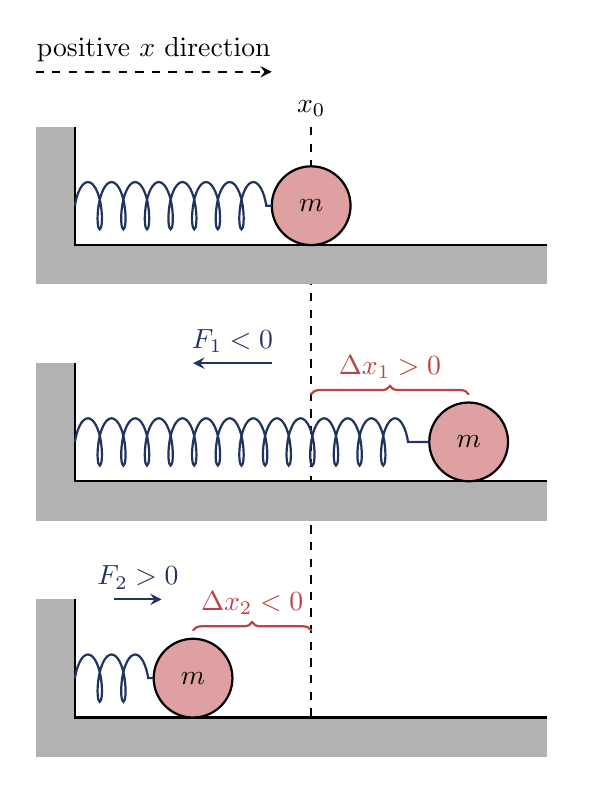
\begin{tikzpicture}
      \coordinate (x0) at (3,1.5);
      \draw[thick, dashed, black] (x0 |- 0,1) node [above] {$x_0$} -- ++(0,-8);
      \draw[thick, dashed,-stealth] (-0.5, 1.7) -- ++(3,0) node [midway, above] {positive $x$ direction};

      \draw[line width=5mm, black!30] (-0.25,1) -- ++(0,-1.75) -- ++(6.25,0);
      \draw[thick] (0,1) -- ++(0,-1.5) -- ++(6,0);
      \draw[thick, fill=xred!50] (3,0) circle (0.5) node (m1) {$m$};
      \draw[springcoil, xdarkblue] (0,0) -- ($(m1)-(0.5,0)$);

      \draw[line width=5mm, black!30] (-0.25,-2) -- ++(0,-1.75) -- ++(6.25,0);
      \draw[thick] (0,-2) -- ++(0,-1.5) -- ++(6,0);
      \draw[thick, fill=xred!50] (5,-3) circle (0.5) node (m2) {$m$};
      \draw[springcoil, xdarkblue] (0,-3) -- ($(m2)-(0.5,0)$);

      \draw[line width=5mm, black!30] (-0.25,-5) -- ++(0,-1.75) -- ++(6.25,0);
      \draw[thick] (0,-5) -- ++(0,-1.5) -- ++(6,0);
      \draw[thick, fill=xred!50] (1.5,-6) circle (0.5) node (m3) {$m$};
      \draw[springcoil, xdarkblue] (0,-6) -- ($(m3)-(0.5,0)$);

      \draw[xred, thick, cap=round, decorate, decoration={brace, amplitude=3pt, raise=3pt}] (m1 |- 0,-2.5) -- (m2 |- 0,-2.5) node[midway, above, yshift=5pt]{$\Delta x_{1}>0$};
      \draw[xred, thick, cap=round, decorate, decoration={brace, amplitude=3pt, raise=3pt, mirror}] (m1 |- 0,-5.5) -- (m3 |- 0,-5.5) node[midway, above, yshift=5pt]{$\Delta x_{2}<0$};

      \draw[-stealth, thick, xdarkblue] (2.5,-2) -- ++(-1,0) node[midway, above] {$F_{1}<0$};
      \draw[-stealth, thick, xdarkblue] (0.5,-5) -- ++(0.6,0) node[midway, above] {$F_{2}>0$};
    \end{tikzpicture}
  \end{center}
  \caption{A simple spring-mass system with spring constant $k$ and a mass $m$. The top figure shows the spring at rest - i.e. when the mass is located at position $x_{0}$ the spring applies no force on the mass (since $\Delta x = x_{m}-x_{0}=0$). The middle figure show the spring being at a \textit{positive} displacement $\Delta x_{1}>0$, causing the spring to pull back with a negative force $F_{1}=-k\Delta x_{1}$. The bottom picture shows the spring contracting by $\Delta x_{2}<0$, casing the spring to apply a positive force $F_{2}=-k\Delta x_{2}$ on the mass.}\label{fig:simple_spring}
\end{figure}

Using Newtons second law of motion (REF?) with $x$ being the displacement from the rest position $x_{0}$, we get the relation
\begin{equation}
  a = -kx,
  \label{eq:simple_spring_newton_2nd_law}
\end{equation}
but since $a = \od{v}{t} = \od[2]{x}{t}$, we can re-write \autoref{eq:simple_spring_newton_2nd_law} as
\begin{equation}
  \od[2]{x}{t} = -kx,
  \label{eq:simple_spring_newton_2nd_law_as_derivative}
\end{equation}
or even more succinctly as
\begin{equation}
  \ddot{x} = -kx.
  \label{eq:simple_spring_newton_2nd_law_as_ddot}
\end{equation}

\autoref{eq:simple_spring_newton_2nd_law_as_ddot} is one of the simplest possible 2nd-order \textit{ordinary} differential equations. Its solution is a combination of the two basic trigonometric equations:
\begin{equation}
  x(t) = c_{1}\sin\left(\alpha t\right) + c_{2}\cos\left(\beta t\right),
  \label{eq:harmonic_solution_ode}
\end{equation}
where $c_{1}$ and $c_{2}$ are constants which we can find using the \textit{starting conditions} (see note \autoref{note:ode_start_cond}), and $\alpha,\beta$ are parameters of the motion. Since function arguments must be unitless, these two parameters also cause the total quantity inside the trigonometric functions to be unitless by having units corresponding to \SIe{1\over time}. For example, if we measure the time in \SIe{\second}, then the units of $\alpha$ and $\beta$ are \SIe{\per\second} = \SIe{\hertz}.

\begin{note}{Starting conditions for solving ODEs}{ode_start_cond}
  Recall that in order to completely solve an ordinary differential equation of order $n$ we must have $n$ starting conditions.
\end{note}

In the case where the initial position of the mass is $x_{0}$ and the initial velocity is $\dot{x}_{0}=0$ we get the simplified solution
\begin{equation}
  x(t) = x_{0}\cos(\omega t),
  \label{eq:harmonic_normal_solution}
\end{equation}
where $\omega=\sqrt{\frac{k}{m}}$. The plot of the position $x(t)$ of the mass is given in \autoref{fig:simple_spring_plot}. Note how, when displayed side-by-side using the same time axes, the position plot is \enquote{lagging behind} the velocity plot by $\phi=\frac{\pi}{2}$: when we start the motion, the velocity is $0$ and then starts to increase in the negative direction (i.e. the mass is moving to the left). The position is at its maximum at that time, and decreases from $x_{\max}$ at $t=0$ to $x=0$ at $t=\frac{\pi}{2}$, while still staying positive. At $t=\frac{\pi}{2}$ the velocity reaches its maximum negative value, $\dot{x}=-v_{\max}$ (which is $1$ in units of $\frac{1}{v_{\max}}$), and the position becomes negative (since it is to the left of the rest position of the spring).

\begin{figure}
  \centering
  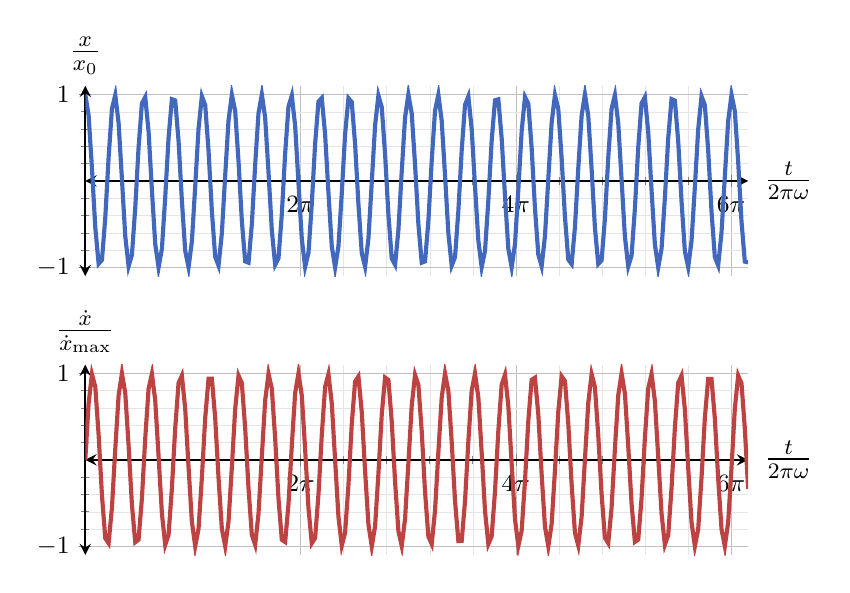
\begin{tikzpicture}
    \begin{axis}[
      name=pos_vs_time,
      graph2d,
      width=10cm, height=4cm,
      xmin=0, xmax=6*pi+0.5,
      ymin=-1.1, ymax=1.1,
      domain={0:6*pi+0.5},
      xlabel=$\frac{t}{2\pi\omega}$,
      ylabel=$\frac{x}{x_{0}}$,
      xtick={2*pi,4*pi,6*pi},
      ytick={-1,0,1},
      xticklabels={$2\pi$,$4\pi$,$6\pi$}
    ]
    \addplot[function={xblue}] {cos(x * 180/pi)};
    \end{axis}
    \begin{axis}[
      at=(pos_vs_time.below south west),
      anchor=north west,
      yshift=-1cm,
      graph2d,
      width=10cm, height=4cm,
      xmin=0, xmax=6*pi+0.5,
      ymin=-1.1, ymax=1.1,
      domain={0:6*pi+0.5},
      xlabel=$\frac{t}{2\pi\omega}$,
      ylabel=$\frac{\dot{x}}{\dot{x}_{\max}}$,
      xtick={2*pi,4*pi,6*pi},
      ytick={-1,0,1},
      xticklabels={$2\pi$,$4\pi$,$6\pi$}
    ]
    \addplot[function={xred}] {-sin(x * 180/pi)};
  \end{axis}
  \end{tikzpicture}
  \caption{Simple harmonic oscillator, top (blue): position $x$ vs. time $t$. The axes units are such that a full period of the oscillation takes $\Delta t=2\pi$, and that the minimum and maximum values of the position are $\pm1$, respectively. Bottom (red): velocity vs. time on the same time axes, and a velocity axis which is scaled such that $v_{\max}=1$.}
  \label{fig:simple_spring_plot}
\end{figure}

It would be useful to understand how does the spring-mass system evolve given a specific combination of position and velocity. This can be done by plotting the \textbf{phase space} of the system (\autoref{fig:harmonic_oscillator_phase_space}): on the horizontal axis we specify the position $x$ of the mass, and on the vertical axis the velocity $\dot{x}$.

\begin{figure}
  \centering
  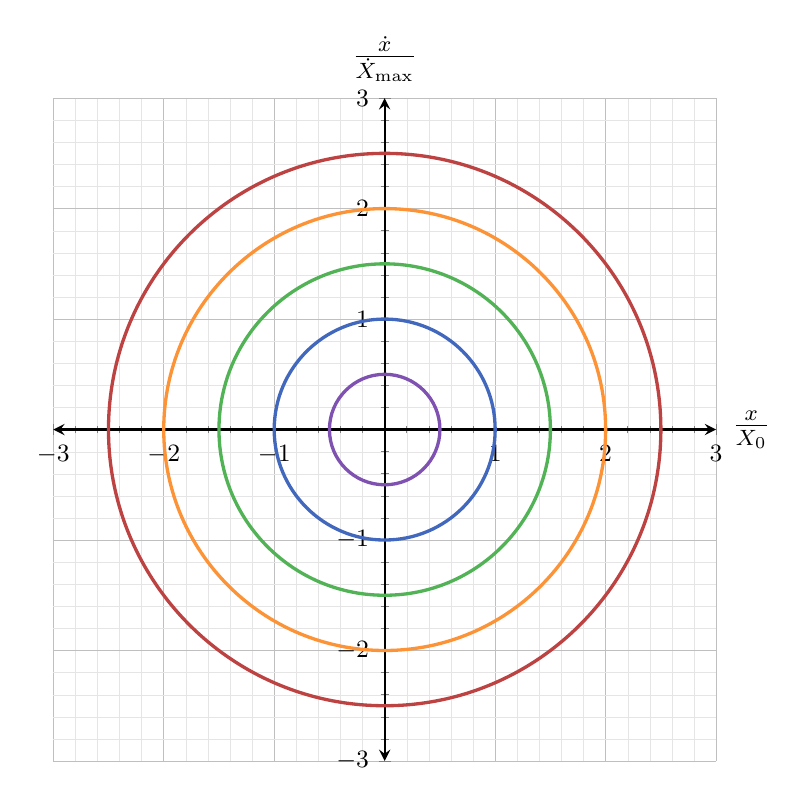
\begin{tikzpicture}
    \begin{axis}[
      graph2d,
      width=10cm, height=10cm,
      xmin=-3, xmax=3,
      ymin=-3, ymax=3,
      axis equal=true,
      domain={-3:3},
      xlabel=$\frac{x}{X_{0}}$,
      ylabel=$\frac{\dot{x}}{\dot{X}_{\max}}$,
      xtick={-3,-2,...,3},
      ytick={-3,-2,...,3},
      samples=100,
    ]
    \draw[very thick, xpurple] (0,0) circle (0.5);
    \draw[very thick, xblue] (0,0) circle (1);
    \draw[very thick, xgreen] (0,0) circle (1.5);
    \draw[very thick, xorange] (0,0) circle (2);
    \draw[very thick, xred] (0,0) circle (2.5);
    \end{axis}
  \end{tikzpicture}
  \caption{Phase space plot of simple harmonic oscillators with different momenta (either their masses are different, or their initial distance are different). The axes are scaled such that their units are the initial position $X_{0}$ and maximum velocity $\dot{X}_{0}$, respectively, of the second oscillator (trajectory drawn in blue).}
  \label{fig:harmonic_oscillator_phase_space}
\end{figure}

In the case of a simple harmonic oscialltor, the evolution of the system is shown on the phase space plot as ellipses - and when we use normalized coordinates ($\tilde{x}=\frac{x}{x_{0}}$ and $\tilde{x}=\frac{\dot{x}}{\dot{X}_{\max}}$), the ellipses turn into perfect circles - just like we see in \autoref{fig:harmonic_oscillator_phase_space}. These circles or ellipses are \underline{paths of constant energy}: this can be seen when we \enquote{translate} the plot to have the potential energy and kinetric energy as horizontal and vertical axes, respectively.

Recall that for close mechanical systems, the total energy $E$ is given by the sum of the sum of the \textit{kinetic energy} $K$ and the \textit{potential energy} $U$:
\begin{equation}
  E = K + U.
  \label{eq:total_energy}
\end{equation}
The kinetic energy is a function of the velocity $v=\dot{x}$:
\begin{equation}
  K = \frac{1}{2}\dot{x}^{2} = \frac{p^{2}}{2m},
  \label{eq:kinetric_energy}
\end{equation}
and the potential energy is a function of the position $x$ via the force $F$:
\begin{equation}
  F = -\od{U}{x}.
  \label{eq:force_from_potential}
\end{equation}
In the case of an harmonic oscillator $F=-kx$, and therefore
\begin{equation}
  U = \int\displaystyle F \dif x = -k\int\displaystyle x \dif x = -\frac{1}{2}kx^{2} + c.
  \label{eq:potential_energy_harmonic_oscillator}
\end{equation}
Since we can add to the potential any constant with no change to the force derived from it (remember that the derivative of a constant is zero), we can simply set the potential at $x=0$ to $U\left(x=0\right)=0$, meaning that the integral constant is $c=0$. Altogether, we get the following system energy:
\begin{equation}
  E = \frac{p}{2m} - \frac{1}{2}kx^{2},
  \label{eq:total_energy_harmonic_oscillator}
\end{equation}
Essentially, this is equal to applying the following transformations to the phase space plot:
\begin{align}
  x &\to -\frac{1}{2}kx^{2},\\
  \dot{x} &\to \frac{p^{2}}{2m} = \frac{1}{2m}{m^{2}\dot{x}^{2}} = \frac{1}{2}m\dot{x}^{2}.
\end{align}
Since the transformation \enquote{streches} both axes by the same power (up to the constants $m$ and $k$), the shapes remain the same as in the original plot.

The total energy of the system can then be extracted from the radius of each circle path:
\begin{equation}
  E = \sqrt{K^{2}+U^{2}} = \sqrt{\frac{p^{2}}{4m^{2}} + \frac{k^{2}x^{4}}{4}} = \frac{1}{2}\left(\frac{p^{2}}{m^{2}}+k^{2}x^{4}\right).
  \label{eq:label}
\end{equation}
When $K=0$ (i.e. $p=0$) the entire energy is stored as potential energy:
\begin{equation}
  E = \frac{1}{2}\sqrt{k^{2}x^{4}} = \frac{1}{2}kx^{2}.
  \label{eq:label}
\end{equation}
And when $U=0$ (i.e. $x=0$) the entire energy is stored as kinetic energy:
\begin{equation}
  E = \frac{1}{2}\sqrt{\frac{p^{2}}{m^{2}}} = \frac{P}{2m} = \frac{1}{2}m\dot{x}^{2}.
  \label{eq:label}
\end{equation}

\subsection{Damped Harmonic Oscillator}
We can make the harmonic oscillator model a bit more realistic if we add a damping force proportional to the velocity of the mass. This corresponds e.g. to introducing friction into the model. The form of the damping force is $F_{\text{damp}}(t)=-cv(t)=-c\dot{x}$, for some real damping coefficient $c\geq0$ (in the case where $c=0$ we get back the simple harmonic oscillator model). Thus, the overall Newton 2nd law equation of the system has the following form:
\begin{equation}
  m\ddot{x} = -c\dot{x}-kx.
  \label{eq:damped_harmonic_oscillator}
\end{equation}

The term $-c\dot{x}$ always acts in the opposite direction to the velocity due to the minus sign. Re-arranging \autoref{eq:damped_harmonic_oscillator} we get the more \enquote{canonical} form
\begin{equation}
  m\ddot{x} + c\dot{x} + kx = 0,
  \label{eq:damped_harmonic_oscillator_different_form}
\end{equation}
We then use the solution $x(t)=\Eu{\lambda t}$, subtituting it into \autoref{eq:damped_harmonic_oscillator_different_form}:
\begin{align}
  F_{\text{total}}(t) &= \lambda^{2}m\Eu{\lambda t} + c\Eu{\lambda t} + k\Eu{\lambda t}\\
  &= \Eu{\lambda t}\left(m\lambda^{2}+c\lambda+k\right)\\
  &= 0.
  \label{eq:2nd_order_ODE_polynomial}
\end{align}

Since \autoref{eq:2nd_order_ODE_polynomial} is true for all $t$ (and in any case $\Eu{\lambda t}\neq 0$ for all $t$), for the equation to be true it must be that the quadratic eqaution in $\lambda$ equals zero. Using the quadratic formula we get that
\begin{equation}
  \lambda_{1,2} = \frac{-c\pm\sqrt{c^{2}-4km}}{2m}.
  \label{eq:2nd_order_ODE_polynomial_solution}
\end{equation}
For the solutions to $\lambda$ to be real numbers, $c^{2}\geq4km$ - otherwise the term in the square root is negative. When $c^{2}>4km$ we call the system \textbf{overdamped}, and the case where $c^{2}=4km$ is the \textbf{critical damping} value. The overall position vs. time relationship of the damped system is given by
\begin{equation}
  x(t) = 
  \label{eq:label}
\end{equation}

\subsection{Simulating Harmonic Oscillators in Python}
Text

\chapter{Mechanics}
\section{Preface}
Text text text

\section{Pendulum}
\subsection{Simple pendulum}
Text text text.

\def\centerarc[#1](#2)(#3:#4:#5)% Syntax: [draw options] (center) (initial angle:final angle:radius)
{ \draw[#1] ($(#2)+({#5*cos(#3)},{#5*sin(#3)})$) arc (#3:#4:#5); }

\begin{figure}
	\begin{center}
		\begin{tikzpicture}
			\pgfmathsetmacro{\th}{45}
			\pgfmathsetmacro{\L}{4}
			\coordinate (origin) at (0,0);
			\coordinate (bob) at ({\L*sin(\th)},{-\L*cos(\th)});
			\draw[stealth-stealth, thick, xblue, dashed] ($(origin)+({4*cos(210)},{4*sin(210)})$) arc (210:330:\L) node [midway, below] {trajectory};
			\draw[thick, fill=black!50] (-1,0) rectangle (1,0.25);
			\draw[thick] (origin) -- (bob) node [midway, above right] {$L$};
			\draw[thick, fill=xgreen!25] (bob) circle (0.5) node {\enquote{bob}};
			\draw[thick, xred, dashed] (origin) -- (0,-3);
			\draw[filledangle={xred}] (origin) -- (0,-1) arc (-90:-\th:1) node [above, pos=0.4] {$\theta$};
		\end{tikzpicture}
	\end{center}
	\caption{A simple pendulum. TBW: add more info.}
	\label{fig:simple_pendulum}
\end{figure}

Using force analysis we can derive an equation of motion for the bob (see \autoref{fig:simple_pendulum_forces}): since the rod can't change its length (it's always $L$), the only variable quantity is the angle $\theta$, and the bob's trajectory is a circle. Any force acting in a radial direction to the trajectory must be counter-balanced (otherwise there will be some acceleration - and therefore motion - in that direction). We are therefore left with only a tangental force, with magnitude
\begin{equation}
	F = -mg\sin(\theta),
	\label{eq:simple_pendulum_tangental_force}
\end{equation}
the minus sign here is chosen to represent that gravity acts in the negative $y$ direction (i.e. \enquote{down}).

Applying Newton's second law we get that
\begin{equation}
	F = ma = -mg\sin(\theta),
	\label{eq:simple_pendulum_newton_second_law}
\end{equation}
i.e.
\begin{equation}
	a = -g\sin(\theta).
	\label{eq:simple_pendulum_acceleration}
\end{equation}

Now we see that the minus sign also makes sense physically, as it shows that the acceleration is always in the opposite direction to the angle (which is negative to the left and positive to the right).

\begin{figure}
	\begin{center}
		\begin{tikzpicture}
			\pgfmathsetmacro{\th}{45}
			\pgfmathsetmacro{\L}{4}
			\coordinate (origin) at (0,0);
			\coordinate (bob) at ({\L*sin(\th)},{-\L*cos(\th)});
			\draw[stealth-stealth, thick, xblue, dashed] ($(origin)+({4*cos(210)},{4*sin(210)})$) arc (210:330:\L);
			\draw[thick, fill=black!50] (-1,0) rectangle (1,0.25);
			\draw[thick] (origin) -- (bob) node [midway, above right] {$L$};
			\draw[thick, fill=xgreen!25] (bob) circle (0.5);
			\draw[vector, xpurple] (bob) -- ++(0,-1.5) node [midway, right] {$\vec{F}_{g}$};
			\draw[vector, xred] (bob) -- ($(bob)!0.3!(origin)$) node [midway, above right] {$\vec{T}$};
			\draw[thick, xred, dashed] (origin) -- (0,-2);
			\draw[filledangle={xred}] (origin) -- (0,-1) arc (-90:-\th:1) node [above, pos=0.4] {$\theta$};
		\end{tikzpicture}
	\end{center}
	\caption{Forces acting on a simple pendulum. TBW: Force compnents.}
	\label{fig:simple_pendulum_forces}
\end{figure}

The tangental position $s$ of the bob can be calculated from the angle $\theta$ by
\begin{equation}
	s = L\theta
	\label{eq:simple_pendulum_tangental_position}
\end{equation}
(recall that $\theta$ is given in radians), and therefore the tangental velocity is
\begin{equation}
	v = \dot{s} = L\dot{\theta},
	\label{eq:simple_pendulum_tangental_velovity}
\end{equation}
and the acceleration is therefore
\begin{equation}
	a = \dot{v} = \ddot{s} = L\ddot{\theta}.
	\label{eq:simple_pendulum_tangental_acceleration}
\end{equation}
Since we know that $a=-g\sin(\theta)$, we get
\begin{equation}
	L\ddot{\theta} = -g\sin(\theta),
\end{equation}
and by moving the rhs term to the left and divide by $l$ we get
\begin{equation}
	\ddot{\theta} + \frac{g}{L}\sin(\theta) = 0.
	\label{eq:simple_pendulum_differential_equation}
\end{equation}

This is a differential equation without analytical solution. We will therefore take two approaches: (1) use an approximation to yield an analytical solution, and (2) solve the equation numerically.

\subsection{Small-angle approximation}
The Taylor series expansion of $\sin(x)$ around $x=0$ is
\begin{equation}
	\sin(x) = x - \frac{1}{3!}x^{3} + \frac{1}{5!}x^{5} - \frac{1}{7!}x^{7} + \dots
	\label{eq:taylor_series_sin}
\end{equation}
We can therefore approximate $\sin(x)$ as $x$ for small values of $x$:
\begin{equation}
	\sin(x) \approx x.
	\label{eq:sin_small_angle_approx}
\end{equation}
This is known as the \enquote{small-angle approximation} of the sine function. By using this approximation we get that the (analytically) unsolvable \autoref{eq:simple_pendulum_differential_equation} reduces to
\begin{equation}
	\ddot{\theta} + \frac{g}{L}\theta = 0,
	\label{eq:simple_pendulum_small_angle_equation}
\end{equation}
for which we have an exact solution:
\begin{equation}
	\theta(t) = A\cos\left(\omega t+\phi\right),
	\label{eq:simple_pendulum_small_angle_solution}
\end{equation}
where $\omega=\sqrt{\frac{g}{L}}$. The parameters $A$ and $\phi$ depend on the initial conditions (i.e. angle and tangental velocity).

TBW: resonance freq, how it looks like (+phase space), python plot?

\subsection{Numerical integration}
Another approach to solve \autoref{eq:simple_pendulum_differential_equation} is doing so numerically, i.e. essentially running a computer simulation. While computers can carry out many calculations per second (in the order of billions, in fact) - they are limited to performing descrete calculations. That is to say, a numerical calculation is also an approximation. However, unlike the small-angle approximation, in principle we can improve the approximation indefinitely, although in practice this is of course impossible.

Let us use a rather naive approach to numerically approximating \autoref{eq:simple_pendulum_differential_equation}: instead of viewing $\theta$ as a continuous function of time $t$, we instead define $t$ to only have equally spaced discrete values $t_{0},t_{1},t_{2},\dots$ such that
\begin{equation}
	t_{n} = t_{0} + n\Delta t,
\end{equation}
or phrased differently: we look at the values $t_{i}$ of $t$ at intervals $\Delta t$ starting from $t_{0}$ (see \autoref{fig:discrete_time}).

\begin{figure}
	\begin{center}
		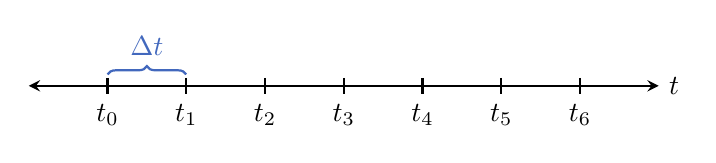
\begin{tikzpicture}
			\draw[stealth-stealth, thick] (-1,0) -- (7,0) node [right] {$t$};
			\foreach \k in {0,1,...,6} {
					\draw[thick] (\k,0.1) -- (\k,-0.1) node [below] {$t_{\k}$};
				}
			\draw[xblue, thick, decorate, decoration={brace, amplitude=3pt, raise=-3pt}]
			(0,0.25) -- ++(1,0) node[midway, above, yshift=0pt]{$\Delta t$};
		\end{tikzpicture}
	\end{center}
	\caption{Discrete time steps.}
	\label{fig:discrete_time}
\end{figure}

In this discrete view, a function of $t$ can also only be evaulated at discrete points. For example, the angle $\theta$ of the bob as a function of time is a discrete function taking the values $\theta_{0},\theta_{1},\theta_{2},\dots$, where each $\theta_{i}$ corresponds to the time $t_{i}$.

How does the discrete angular velocity look like in this scheme? It's worth looking at the definition of angular velocity in the continuous case:
\begin{equation}
	\omega(t) = \dot{\theta}(t) = \od{\theta(t)}{t} = \lim\limits_{\Delta t\to0}\frac{\theta\left(t+\Delta t\right)-\theta(t)}{\Delta t}.
	\label{eq:label}
\end{equation}
To descritize, we can replace $\theta(t)$ with $\theta_{t_{i}}=\theta_{i}$, and therefore $\theta\left(t+\Delta t\right)$ with $\theta_{t_{i}+\Delta t}=\theta_{i+1}$. The limit $\lim\limits_{\Delta t\to 0}$ is pretty meaningless, since the smallest $\Delta t$ possible in the discrete case is the $\Delta t$ we chose to discretize out time steps. Therefore, we get that the discrete version of $\omega(t)$ is
\begin{equation}
	\omega_{i} = \frac{\theta_{i+1}-\theta_{i}}{\Delta t},
	\label{eq:discrete_velocity}
\end{equation}
which is nothing more than saying that the angular velocity at time $t_{i}$ is simply the difference between the angle at time $t_{i+1}$ and the angle at time $t_{i}$, divided by the time difference $\Delta t$.

\autoref{eq:discrete_velocity} gives us a powerful tool: if we only know the current angle $\theta_{i}$ of the bob and its current velocity $\omega_{i}$, then its next position $\theta_{i+1}$ is a simple rearrangement of the equation:
\begin{equation}
	\theta_{i+1} = \theta_{i} + \omega_{i}\Delta t.
	\label{eq:next_position_from_velocity}
\end{equation}

The same logic can be applied to the angular acceleration $\alpha(t)$: in the continuous version its given by
\begin{equation}
	\alpha(t) = \dot{\omega(t)} = \od{\omega(t)}{t} = \lim\limits_{\Delta t\to 0}\frac{\omega\left(t+\Delta t\right)-\omega(t)}{\Delta t},
\end{equation}
and thus the discrete version is
\begin{equation}
	\alpha_{i} = \frac{\omega_{i+1}-\omega_{i}}{\Delta t},
\end{equation}
and recovering the angular velocity $\omega_{i+1}$ from the angular velocity $\omega_{i}$ and the angular acceleration $\alpha_{i}$ is done by
\begin{equation}
	\omega_{i+1} = \omega_{i}+\alpha_{i}\Delta t.
	\label{eq:next_velocity_from_acceleration}
\end{equation}

Since we use the inverse of the differentiation operation (in the discrete sense) to recover the quantity we're after, this scheme is known as a \textbf{numerical integration}. Specifically, this kind of numerical integration is called the \textbf{Forward-Euler} method, and it is generally considered unfavourable due to the fast rate with which it gains errors, and is rarely used in practice.

However, for the sake of simplicity of writing our first simulations, we will not discuss these issues now, nor will we generalize the method and present better ones - both of which we will do later in the course. Instead, for now we will continue with using this method to devise a numerical integration scheme for a simple pendulum.

In the case of the pendulum, recall that the acceleration at time $t$ is $\ddot{\theta}(t)=-\frac{g}{L}\sin(\theta)$ (\autoref{eq:simple_pendulum_differential_equation}), and therefore we can discretize it as
\begin{equation}
	\alpha_{i+1} = -\frac{g}{L}\sin\left(\theta_{i}\right).
	\label{eq:pendulum_discrete_acceleration}
\end{equation}
%%% !!! TBW: why alpha_{i+1} instead of alpha_{i} !!! %%%
We then use the forward Euler method to get the angular velocity and angle, as seen in \autoref{eq:next_velocity_from_acceleration} and \autoref{eq:next_position_from_velocity}, respectively.
%%% Add code example redirection, maybe a nice tcolorbox?

\subsection{Damped oscillation}
A slightly more realistic model of a pendulum also considers the way the pendulum loses energy over time (e.g. via friction). This can be modelled by adding a force which resists the angular velocity (see also \autoref{fig:pendulum_damping_force}):
\begin{equation}
	F_{d} = -bL\dot{\theta},
	\label{eq:damping_force}
\end{equation}
where $b$ is simply a parameter which adjusts how strong the damping is.

\begin{figure}
	\begin{center}
		\begin{tikzpicture}
			\pgfmathsetmacro{\th}{25}
			\pgfmathsetmacro{\L}{4}
			\coordinate (origin) at (0,0);
			\coordinate (bob) at ({\L*sin(\th)},{-\L*cos(\th)});
			\draw[stealth-stealth, thick, xblue, dashed, opacity=0.25] ($(origin)+({4*cos(210)},{4*sin(210)})$) arc (210:330:\L);
			\draw[thick, fill=black!50] (-1,0) rectangle (1,0.25);
			\draw[thick] (origin) -- (bob) node [midway, above right] {$L$};
			\draw[thick, fill=xgreen!25] (bob) circle (0.5);
			\draw[vector, xpurple] (bob) -- ++(0,-1.5) node [midway, right] {$\vec{F}_{g}$};
			\draw[vector, xred] (bob) -- ($(bob)!0.3!(origin)$) node [midway, above right] {$\vec{T}$};
			\draw[thick, xred, dashed] (origin) -- (0,-2);
			\draw[filledangle={xred}] (origin) -- (0,-1) arc (-90:{-90+\th}:1) node [above, pos=0.4] {$\theta$};
			\draw[vector, xblue] (bob) -- ++({-1.5*cos(\th)},{-1.5*sin(\th)}) node [pos=1.2] {$\vec{v}$};
			\draw[vector, xorange] (bob) -- ++({1*cos(\th)},{1*sin(\th)}) node [pos=1.2] {$\vec{F}_{d}$};
		\end{tikzpicture}
	\end{center}
	\caption{Forces on a pendulum including a damping force.}
	\label{fig:pendulum_damping_force}
\end{figure}

Using Newton's second law, recalling that $a=L\ddot{\theta}$ (\autoref{eq:simple_pendulum_tangental_acceleration}), we get
\begin{equation}
	mL\ddot{\theta} = F_{g} + F_{d} = -mg\sin(\theta) - bL\dot{\theta}.
	\label{eq:damped_pendulum_differential_equation}
\end{equation}

It's common to use $\beta=\frac{b}{2m}$ and of course $\omega_{0}=\sqrt{\frac{g}{L}}$, which together with some rearrangement gives us
\begin{equation}
	\ddot{\theta} = -2\beta\dot{\theta} -\omega_{0}^{2}\sin(\theta).
	\label{eq:damped_pendulum_differential_equation_2}
\end{equation}

%%% TBW: under/over/critical-damping, etc.

\subsection{Double pendulum}
An interesting system arises when we take a simple pendulum and attach another simple pendulum to it (as seen in \autoref{fig:double_pendulum}): unlike a simple pendulum, this system exhibits very complex dynamics which is sensitive to the initial conditions - i.e. it is \textbf{chaotic}, meaning that small changes in the initial conditions evolve into big differences in the dynamics of the system.

\begin{figure}
	\begin{center}
		\begin{tikzpicture}
			\pgfmathsetmacro{\thA}{30}
			\pgfmathsetmacro{\LA}{3}
			\pgfmathsetmacro{\thB}{55}
			\pgfmathsetmacro{\LB}{2.5}
			\coordinate (origin) at (0,0);
			\coordinate (bobA) at ({\LA*sin(\thA)},{-\LA*cos(\thA)});
			\coordinate (bobB) at ($(bobA)+({\LB*sin(\thB)},{-\LB*cos(\thB)})$);
			\draw[thick, fill=black!50] (-1,0) rectangle (1,0.25);
			\draw[thick, xred, dashed] (origin) -- ++(0,-1.5);
			\draw[filledangle={xred}] (origin) -- ++(0,-1) arc (-90:{-90+\thA}:1) node [above, pos=0.4] {$\theta_{1}$};
			\draw[thick, xpurple, dashed] (bobA) -- ++(0,-1.5);
			\draw[filledangle={xpurple}] (bobA) -- ++(0,-1) arc (-90:{-90+\thB}:1) node [above, pos=0.4] {$\theta_{2}$};
			\draw[thick] (origin) -- (bobA) node [midway, above right] {$L_{1}$};
			\draw[thick] (bobA) -- (bobB) node [midway, above right] {$L_{2}$};
			\draw[thick, fill=xgreen!25] (bobA) circle (0.35) node {$m_{1}$};
			\draw[thick, fill=xblue!25 ] (bobB) circle (0.35) node {$m_{2}$};
		\end{tikzpicture}
	\end{center}
	\caption{A double pendulum. TBW: add more info.}
	\label{fig:double_pendulum}
\end{figure}

To analyze the behaviour of the system we again seek to find a differntial equation which will describe the system completely. Unfortunately, this differential equation is rather complicated and is composed of two coupled differential equations. We will only present the equation here but not how to derive it - this will be added in an appendix.

The differential equations governing the dynamics of the system are:
\begin{equation}
	\begin{aligned}
		0 & = \left(m_{1}+m_{2}\right)L_{1}\ddot{\theta}_{1} + m_{2}L_{2}\ddot{\theta}_{2}\cos\left(\theta_{1}-\theta_{2}\right) + m_{2}L_{2}\dot{\theta}_{2}^{2}\sin\left(\theta_{1}-\theta_{2}\right) \\
		  & + \left(m_{1}+m_{2}\right)g\sin\left(\theta_{1}\right),
	\end{aligned}
\end{equation}
and
\begin{equation}
	0 = L_{2}\ddot{\theta}_{2}+L_{1}\ddot{\theta}_{1}\cos\left(\theta_{1}-\theta_{2}\right) - L_{1}\dot{\theta}_{1}^{2}\sin\left(\theta_{1}-\theta_{2}\right) + g\sin\left(\theta_{2}\right).
\end{equation}

To help us get excplicit expressions for $\ddot{\theta}_{1}$ and $\ddot{\theta}_{2}$ we can define the following quantities:
\begin{equation}
	\alpha = \frac{m_{2}}{m_{1}},\quad \beta = \frac{L_{2}}{L_{1}},\quad \gamma = \frac{g}{L_{1}},\quad \Delta\theta = \theta_{1}-\theta_{2}.
	\label{eq:double_pendulum_helper_defs}
\end{equation}
we then get the following \enquote{beautiful} expressions for $\ddot{\theta}_{1}$ and $\ddot{\theta}_{2}$:
\begin{align}
	\begin{split}
		\ddot{\theta}_{1} & = -\frac{\left(1+\alpha\right)\gamma\sin\left(\theta_{1}\right) + \alpha\beta\dot{\theta}_{2}^{2}\sin(\Delta\theta)+\alpha\cos\left(\Delta\theta\right)\left[\dot{\theta}_{1}^{2}\sin\left(\Delta\theta\right)-\gamma\sin\left(\theta_{2}\right)\right]}{1+\alpha\sin^{2}\left(\Delta\theta\right)},                                                       \\
		\ddot{\theta}_{2} & = \frac{\left(1+\alpha\right)\left(\dot{\theta}_{1}^{2}\sin\left(\Delta\theta\right)-\gamma\sin\left(\theta_{2}\right)+\cos\left(\Delta\theta\right)\left[\left(1+\alpha\right)\gamma\sin\left(\theta_{1}\right)+\alpha\beta\dot{\theta}^{2}_{2}\sin\left(\Delta\theta\right)\right]\right)}{\beta\left[1+\alpha\sin^{2}\left(\Delta\theta\right)\right]}.
	\end{split}
	\label{eq:double_pendulum_accelerations}
\end{align}

\newcommand{\Si}{\text{S}}
\newcommand{\Co}{\text{C}}
Discretizing \autoref{eq:double_pendulum_accelerations} can then be done as following: first,
\begin{enumerate}
	\item $\alpha,\ \beta$ and $\gamma$ are defined as in \autoref{eq:double_pendulum_helper_defs}.
	\item Set $\Delta\theta_{k} = \theta_{1,k} - \theta_{2,k}$.
	\item For compactness, we set $N_{k} = 1+\alpha\sin^{2}\left(\Delta\theta_{k}\right)$, $\Si(x)=\sin(x)$, $\Co(x)=\cos(x)$ and $A=1+\alpha$.
\end{enumerate}
Then, we get
\begin{align}
	\begin{split}
		\ddot{\theta}_{1,i} & = -\frac{A\gamma\Si(\theta_{1,i-1})+\alpha\beta\dot{\theta}_{2,i-1}^{2}\Si\left(\Delta\theta_{i-1}\right) + \alpha\Co\left(\Delta\theta_{i-1}\right)\left[\dot{\theta}_{1,i-1}^{2}\Si\left(\Delta\theta_{i-1}\right)-\gamma\Si\left(\theta_{2,i-1}\right)\right]}{N_{i-1}},                       \\
		\ddot{\theta}_{2,i} & = \frac{A\left(\dot{\theta}_{1,i-1}^{2}\Si\left(\Delta\theta_{i-1}\right)-\gamma\Si\left(\theta_{2,i-1}\right)+\Co\left(\Delta\theta_{i-1}\right)\left[A\gamma\Si\left(\theta_{1,i-1}\right)+\alpha\beta\dot{\theta}_{2,i-1}^{2}\Si\left(\Delta\theta_{i-1}\right)\right]\right)}{\beta N_{i-1}}.
	\end{split}
\end{align}
(lovely, isn't it?)

% \section{Orbital Mechanics}
% \subsection{Classic Gravitational Force}
% Already in the 17th century, \textit{Isaac Newton} formulated the gravitational force existing between any two objects with masses greater than zero. The strength of the force is given by the equation
% \begin{equation}
% 	F = G\frac{m_{1}m_{2}}{r^{2}},
% 	\label{eq:force_gravity}
% \end{equation}
% where $m_{1}$ and $m_{2}$ are the respective masses of the two objects, $r$ is the distance between them, and $G$ is a the \textit{universal gravitational constant},
% \begin{equation}
% 	G = \SI{6.6743(15)e-11}{\newton\metre\squared\per\kg\squared}
% 	\label{eq:universal_gravity_constant}
% \end{equation}
%
% The direction of the force is the line connecting the centers of mass of the two objects. Due to Newton's third law, the forces acting on the two objects are equal and opposite: the force applied by $m_{1}$ on $m_{2}$, $F_{1\to2}$, is pointing \textbf{from} $m_{2}$ \textbf{onto} $m_{1}$, and the force applied by $m_{2}$ on $m_{1}$, $F_{2\to1}$ is pointing \textbf{from} $m_{1}$ \textbf{onto} $m_{2}$ - and is exactly opposite to $F_{1\to2}$, i.e. in vector notation
% \begin{equation}
% 	\vec{F}_{1\to2} = -\vec{F}_{2\to1}.
% 	\label{eq:gravity_force_vector_directions}
% \end{equation}
%
% If the two objects have positions $\vec{r}_{1}$ and $\vec{r}_{2}$, the vector pointing from object $1$ to object $2$ is
% \begin{equation}
% 	\vec{r}_{1\to2} = \vec{r}_{2} - \vec{r}_{1},
% 	\label{eq:position_vector}
% \end{equation}
% with the vector pointing from object $2$ to object $1$ having the exact opposite components, i.e. $\vec{r}_{2\to1}=-\vec{r}_{1\to2}$. The norms of $\vec{r}_{1\to2}$ and $\vec{r}_{2\to1}$ are simply $r$ (the distance between the objects), and their directions are the unit vectors in the direction of $\vec{r}_{1\to2}$ and $\vec{r}_{2\to1}$, respectively:
% \begin{align}
% 	\uvec{r}_{1\to2} & = \frac{\vec{r}_{1\to2}}{\vnorm{r}_{1\to2}} = \frac{\vec{r}_{1\to2}}{r}\nonumber,           \\
% 	\uvec{r}_{2\to1} & = \frac{\vec{r}_{2\to1}}{\vnorm{r}_{2\to1}} = \frac{\vec{r}_{2\to1}}{r} = -\uvec{r}_{1\to2}.
% 	\label{eq:normed_position_vector}
% \end{align}
%
% \begin{figure}
% 	\begin{center}
% 		\begin{tikzpicture}
% 			\pgfmathsetmacro{\a}{4}
% 			\pgfmathsetmacro{\b}{2}
% 			\coordinate (m1) at (0,0);
% 			\coordinate (m2) at (\a,\b);
% 			\coordinate (dp) at (-\b, \a);
% 			\coordinate (l1) at ($(m1)!1.3cm!(dp)$);
% 			\coordinate (l2) at ($(m2) + (m1)!1.3cm!(dp)$);
% 			\def\R{1cm}
% 			\def\r{0.5cm}
% 			\def\F{0.8cm}
% 			\draw[vector, xred, dashed] ($(m1)+(m1)!\R!(m2)$) -- ++($(m1)!\F!(m2)$) node[midway, below right, xshift=-1mm] {$\vec{F}_{2\to1}$};
% 			\draw[vector, xgreen, dashed] ($(m2)-(m1)!\r!(m2)$) -- ++($(m1)!-\F!(m2)$) node[midway, above left, xshift=1mm] {$\vec{F}_{1\to2}$};
% 			\draw[thick, fill=xgreen!50] (m1) circle (\R) node {$m_{1}$};
% 			\draw[thick, fill=xred!50] (m2) circle (\r) node {$m_{2}$};
% 			\draw[thick, cap=round, decorate, decoration={brace, amplitude=5pt}] (l1) -- (l2) node[midway, above left, xshift=0mm, yshift=2mm]{$r$};
% 			\draw[thick, densely dotted, black!75] ($(m1)+(m1)!0.15!(l1)$) -- (l1);
% 			\draw[thick, densely dotted, black!75] ($(m2)+(m1)!0.15!(l1)$) -- (l2);
% 		\end{tikzpicture}
% 	\end{center}
% 	\caption{Gravitational force between two objects with masses $m_{1}$ and $m_{2}$. Each object applies an attrctive force on the other object, with norm $F=G\frac{m_{1}m_{2}}{r^{2}}$ (where $r$ is the distance between the objects) and in the direction pointing from each object to the other object.}
% 	\label{fig:gravity_basics}
% \end{figure}
%
% In total, the vector notation of the gravitational force applied by the objects on each other are
% \begin{align}
% 	\vec{F}_{1\to2} & = Gm_{1}m_{2}\frac{\uvec{r}_{1\to2}}{r^{2}}\nonumber,           \\
% 	\vec{F}_{2\to1} & = Gm_{1}m_{2}\frac{\uvec{r}_{2\to1}}{r^{2}} = -\vec{F}_{1\to2}.
% 	\label{eq:gravity_forces_vector_notation}
% \end{align}
%
% \begin{note}{Another gravity force vector notation}{}
% 	In some textbooks, \autoref{eq:gravity_forces_vector_notation} are written without the unit vectors $\uvec{r}_{1\to2}$ and $\uvec{r}_{2\to1}$, instead using the distance vectors and dividing by $r^{3}$, i.e.
% 	\begin{align*}
% 		\vec{F}_{1\to2} & = Gm_{1}m_{2}\frac{\vec{r}_{1\to2}}{r^{3}}, \\
% 		\vec{F}_{2\to1} & = Gm_{2}m_{1}\frac{\vec{r}_{2\to1}}{r^{3}}.
% 	\end{align*}
% 	The result is of course the same as in \autoref{eq:gravity_forces_vector_notation}, since for any non zero vector $\vec{v}$,
% 	\begin{align*}
% 		\frac{\vec{v}}{\vnorm{v}^{3}} = \frac{1}{\vnorm{v}^{2}}\frac{\vec{v}}{\vnorm{v}} = \frac{1}{\vnorm{v}^{2}}\uvec{v}.
% 	\end{align*}
% \end{note}
%
% Let us look at an example of calculating the gravitational forces between two objects.
%
% \begin{example}{Calculating a gravitational force}{grav_force_2_objects}
% 	Let us calculate the gravitational forces between two objects $A$ and $B$, using the following parameters:
% 	\begin{align*}
% 		\vec{r}_{A} & =\colvec{1;-2;0},\ m_{A} = 1, \\
% 		\vec{r}_{B} & =\colvec{2;5;-2},\ m_{B} = 2.
% 	\end{align*}
% 	For the sake of simplicity, we use $G=1$ and don't consider units with this example.
%
% 	The vector pointing from $A$ to $B$ is
% 	\[
% 		\vec{r}_{A\to B} = \vec{B}-\vec{A} = \colvec{2;5;-2} - \colvec{1;-2;0} = \colvec{1;7;-2},
% 	\]
% 	and the vector pointing from $B$ to $A$ is
% 	\[
% 		\vec{r}_{B\to A} = -\vec{r}_{A\to B} = \colvec{-1;-7;2}.
% 	\]
%
% 	The disntace $r$ between the objects is the norm of either of the above vectors, so we'll use $\vec{r}_{A\to B}$:
% 	\[
% 		r = \vnorm{r}_{A\to B} = \sqrt{1^{2}+7^{2}+2^{2}} = \sqrt{19} \approx 7.3485.
% 	\]
%
% 	The direction vectors are therefore
% 	\begin{align*}
% 		\uvec{r}_{A\to B} & = \frac{1}{7.3485}\colvec{1;7;-2} = \colvec{0.1361;0.9526;-0.2722}, \\
% 		\uvec{r}_{B\to A} & = -\uvec{r}_{A\to B} = \colvec{-0.1361;-0.9526;0.2722}.
% 	\end{align*}
%
% 	The gravity force which $A$ applies onto $B$ is then
% 	\[
% 		\vec{F}_{A\to B} = \cancel{G}\frac{\overbrace{m_{1}m_{2}}^{=2\times1}}{r^{2}}\uvec{r}_{A\to B} = \frac{2}{54}\colvec{0.1361;0.9526;-0.2722} = \colvec{0.0050;0.0353;-0.101}.
% 	\]
% 	and similarily,
% 	\[
% 		\vec{F}_{B\to A} = -\vec{F}_{A\to B} = \colvec{-0.0050;-0.0353;0.101}.
% 	\]
% \end{example}
%
% In the case where we only consider two objects, and choose our frame of reference such that one of the objects is stationary - an analytical solution to the spatial trajectory taken by the second object is known and well studied. It is called a \textbf{Keplerian orbit}, and it always takes the form of a conic section. Let us take a short detour to discuss conic sections.
%
% \subsection{Conic Sections}
% A conic section (sometimes simply just called \enquote{a conic}) is a 2-dimensional shape resulting from the intersection of a plane and a cone (see \autoref{fig:3d_conic_1}). Depending on the angle $\alpha$ by which the plane intersects the cone relative to the the cone's side, the resulting shape can be one of 3 general types (here $\theta$ is the cone's angle):
% \begin{enumerate}
% 	\item If $\alpha>\theta$ the intersection is an \textbf{ellipse}. If in addition $\alpha=\ang{90}$ the ellipse becomes a \textbf{circle}.
% 	\item If $\alpha=\theta$ the intersection is a \textbf{parabola}.
% 	\item If $\alpha<\theta$ the intersection is a \textbf{hyperbola}.
% \end{enumerate}
%
% \begin{figure}
% 	\begin{center}
% 		
\includegraphics[scale=0.65]{figs/mechanics/cone_plane_3d.pdf}
% 	\end{center}
% 	\caption{An intersection of a cone and a plane. Both the cone and plane are infinite - the cone extends infinitely \enquote{down}, but also has a second \enquote{inverted} part on the top, also extending to infinity. In the case here shown, the intersection is an ellipse. Image reproduced with modifications from !SOURCE!} % source: https://latexdraw.com/draw-a-plane-intersecting-a-cone-in-latex/
% 	\label{fig:3d_conic_1}
% \end{figure}
%
% \begin{figure}
% 	\begin{center}
% 		\begin{tikzpicture}
% 			\pgfmathsetmacro{\Lth}{1}
% 			\pgfmathsetmacro{\x}{2.25}
% 			\pgfmathsetmacro{\y}{3.5}
% 			\pgfmathsetmacro{\th}{atan(\y/\x)}
% 			\coordinate (h1) at (0,0);
% 			\coordinate (h2) at (0,-\y);
%
% 			% Cone
% 			\draw[filledangle={xpurple}] (h1) -- (0,-\Lth) arc (-90:-\th:\Lth) node [above, pos=0.37] {$\theta$};
% 			\draw[thick] (h1) -- (\x,-\y);
% 			\draw[thick] (h1) -- (-\x,-\y);
% 			\draw[thick, dashed, black!75] (-\x,-\y) -- ($(-\x,-\y)!1.4!(h1)$);
% 			\draw[thick] (-\x,-\y) -- ($(-\x,-\y)!1.2!(h1)$) node[above left, pos=0.6] {$C$};
% 			\draw[thick, dashed, black!75] (\x,-\y) -- ($(\x,-\y)!1.4!(h1)$);
% 			\draw[thick] (\x,-\y) -- ($(\x,-\y)!1.2!(h1)$);
% 			\draw[thick, dashed, black!75] (0,-\y) -- ($(0,-\y)!1.25!(h1)$) node[right, pos=0.05] {$h$};
%
% 			% Plane
% 			\pgfmathsetmacro{\px}{2}
% 			\pgfmathsetmacro{\pya}{1.25}
% 			\pgfmathsetmacro{\pyb}{2.25}
% 			\pgfmathsetmacro{\alph}{atan((\pyb-\pya)/(2*\px))}
% 			\pgfmathsetmacro{\Lalph}{0.75}
% 			\coordinate (p1) at (-\px,-\pya);
% 			\coordinate (p2) at (\px,-\pyb);
% 			\draw[thick, xred, dashed] (p1) -- ($(p1)!-0.2!(p2)$);
% 			\draw[thick, xred, dashed] (p2) -- ($(p1)!1.2!(p2)$);
% 			\draw[thick, xred, name path=p1--p2] (p1) -- (p2) node[above, pos=0.95] {$P$};
% 			\draw[name path=h1--h2, opacity=0] (h1) -- (h2);
% 			\path[name intersections={of=p1--p2 and h1--h2, by=E}];
% 			\draw[filledangle={xblue}] (E) -- ++(0,-\Lalph) arc (-90:-\alph:\Lalph) node[above, pos=0.35] {$\alpha$};
% 		\end{tikzpicture}
% 	\end{center}
% 	\caption{Side view of an infinite cone $C$ and an infinite plane $P$ intersecting it. The angle between $P$ and the cone's height line $h$ is $\alpha$, and the angle between the cone's surface and $h$ is $\theta$. In this figure $0<\theta<\alpha<\ang{90}$, and thus the shape formed by the intersection of $C$ and $P$ is an ellipse.}
% 	\label{fig:cone_side_view}
% \end{figure}
%
%
% Depending on the exact parameters of both $C$ and $P$, the resulting conic section can be \textbf{degenerate} - either a point, a line or two intersection lines. This happens if $P$ goes throgh the vertex point of $C$: if $\alpha=\ang{90}$ the result is a single point \footnote{one can understand this as being a circle with radius $r=0$.}, if $\alpha=\theta$ the result is a single line, and if $\alpha>\theta$ the result is two intersecting lines.
%
% \subsection{Geometric Properties of Conic Sections}
% Of the non-degenerate conic sections, the ellipse is the only closed curve. Both the parabola and hyperbola are open: in essence, this means that they diverge to infinity. A common geometric definition for all conic sections is the following: given a line $L$ (called the \textbf{directrix}) and a point $F$ (called the \textbf{locus}), a conic section is the set $C$ of all points $\left\{p\right\}$ for which the distance $Fp$ is equal to a constant multiple of the distance $Lp$:
% \begin{equation}
% 	C = \left\{ p \mid \snorm{Fp} = e\snorm{Lp} \right\}.
% 	\label{eq:conic_section_geometric_definition}
% \end{equation}
% The constant $e$ is called the \textbf{eccentricity} of the conic section.
%
% \begin{figure}
% 	\begin{center}
% 		\begin{tikzpicture}
% 			\begin{axis}[
% 					graph2d,
% 					width=12cm, height=12cm,
% 					xmin=-2, xmax=2,
% 					ymin=-2, ymax=2,
% 					restrict y to domain=-3:3,
% 					xticklabels={,},
% 					yticklabels={,},
% 					cycle list/Spectral,
% 					declare function={
% 							conic(\x,\A,\E) = \A*(\E+\A)/(1+\E*cos(\x));
% 						},
% 				]
% 				\pgfmathsetmacro{\A}{0.5}
% 				\foreach \E in {0.0,0.1,...,5,5.5,...,10} {
% 						\edef\drawconic{\noexpand\addplot[black!5, very thick, data cs=polar, domain=0:2*pi, samples=100, smooth] (x,{conic(x,\A,\E)});}
% 						\drawconic
% 					}
% 				\foreach \E in {0,0.25,...,1,2,...,5} {
% 						\edef\drawconic{\noexpand\addplot+[very thick, data cs=polar, domain=0:2*pi, samples=100, smooth] (x,{conic(x,\A,\E)});}
% 						\drawconic
% 					}
% 				% \addplot[function={xred}] ()
% 			\end{axis}
% 		\end{tikzpicture}
% 	\end{center}
% 	\caption{Several conic sections with different eccentricities $\left\{e_{i}\right\}$ and the same locus $F$ and directrix $L$. (NOTE: figure still WIP)}
% 	\label{fig:conic_sections_geometrically}
% \end{figure}
%
% MORE TEXT HERE
%
% \subsection{Cartesian coefficients}
% All conic sections can be expressed as the solutions to the following general equation in $\Rs[2]$:
% \begin{equation}
% 	Ax^{2}+Bxy+Cy^{2}+Dx+Ey+F=0,
% 	\label{eq:conic_section_cartesian_form}
% \end{equation}
% where $A, B, C, D, E, F$ are all real coefficients such that $A, B$ and $C$ are all nonzero. The above equation can be written in matrix form as
% \begin{equation}
% 	\rowvec{x;y;1}
% 	\begin{bmatrix}
% 		A   & B/2 & D/2 \\
% 		B/2 & C   & E/2 \\
% 		D/2 & E/2 & F
% 	\end{bmatrix}
% 	\colvec{x;y;1}=0.
% 	\label{eq:conic_section_cartesian_form_matrix}
% \end{equation}
%
% In this form, the different typs of conic sections arise from the sign of the term
% \begin{equation}
% 	\Delta = B^{2}-4AC,
% 	\label{eq:conic_section_discriminant}
% \end{equation}
% called the \textbf{discriminent} of the conic equation, as following:
% \begin{enumerate}
% 	\item If $B^{2}-4AC<0$ the equation represents an ellipse. If in addition $A=C$ and $B=0$ the discriminent collapses to $-A^{2}$ - which represents a circle.
% 	\item If $B^{2}-4AC=0$, the equation represents a parabola.
% 	\item If $B^{2}-4AC>0$, the equation represents a hyperbola.
% \end{enumerate}
%
% Note that the discriminent can be represented as a $2\times2$ determinant derived from the matrix form of the Cartesian coefficients:
% \begin{equation}
% 	\Delta = -4\begin{vmatrix} A & B/2 \\ B/2 & C \end{vmatrix}.
% 	\label{eq:conic_section_discriminant_as_determinant}
% \end{equation}
%
% \subsection{Conic Section From 5 Points}
% If we know 5 points lying on a conic,
% \begin{equation}
% 	\begin{cases}
% 		\bm{p}_{1}=\left(x_{1},y_{1}\right) \\
% 		\bm{p}_{2}=\left(x_{2},y_{2}\right) \\
% 		\vdots                              \\
% 		\bm{p}_{5}=\left(x_{5},y_{5}\right),
% 	\end{cases}
% 	\label{eq:5_points_on_conic}
% \end{equation}
% we can determine all the conic Cartesian coefficients by solving the equation
% \begin{equation}
% 	\begin{bmatrix}
% 		x_{1}^{2} & x_{1}y_{1} & y_{1}^{2} & x_{1} & y_{1} & 1 \\
% 		x_{2}^{2} & x_{2}y_{2} & y_{2}^{2} & x_{2} & y_{2} & 1 \\
% 		x_{3}^{2} & x_{3}y_{3} & y_{3}^{2} & x_{3} & y_{3} & 1 \\
% 		x_{4}^{2} & x_{4}y_{4} & y_{4}^{2} & x_{4} & y_{4} & 1 \\
% 		x_{5}^{2} & x_{5}y_{5} & y_{5}^{2} & x_{5} & y_{5} & 1
% 	\end{bmatrix}
% 	\colvec{A;B;C;D;E;F} = \colvec{0;0;0;0;0},
% 	\label{eq:5_points_determine_conic_matrix_equation}
% \end{equation}
% which can be done by finding the null space of the matrix in the above equation.
%
% \subsection{Some More About Ellipses}
% Unlike the other conic sections, an ellipse has two focus points (simply called its \textbf{foci}): $F_{1}$ and $F_{2}$. One of these always corresponds to the conic section definition of the focus. In an ellipse, the sum of the distances from any point to the two foci is always constant. In a sense, an ellipse is an elognated circle: instead of having a single radius, it has two orthogonal \textbf{axes}: the semi-major axis $a$ and the semi-minor axis $b$ (such that $a\geq b$).
%
% \begin{figure}
% 	\begin{center}
% 		\begin{tikzpicture}
% 			\pgfmathsetmacro{\a}{5.5}
% 			\pgfmathsetmacro{\b}{3.5}
% 			\pgfmathsetmacro{\c}{\a*sqrt(1-(\b/\a)^2)}
%
% 			% Drawings
% 			\draw[ultra thick, xred] (0,0) ellipse [x radius=\a, y radius=\b];
% 			\node[point={}] (C) at (0,0) {};
% 			\node[point={}] (pa1) at (\a,0) {};
% 			\node[point={}] (pa2) at (-\a,0) {};
% 			\node[point={}] (pb1) at (0,\b) {};
% 			\node[point={}] (pb2) at (0,-\b) {};
% 			\draw[thick, dashed, black!75] (pa1) -- (pa2);
% 			\draw[thick, dashed, black!75] (pb1) -- (pb2);
% 			\draw[ultra thick, xgreen] (C) -- (pb1) node[midway, below, rotate=90] {semi-minor axis, $b$};
% 			\node[point={$F_{1}$}] (F1) at (\c,0) {};
% 			\node[point={$F_{2}$}] (F2) at (-\c,0) {};
% 			\draw[ultra thick, xpurple] (F2) -- (C) node[pos=0.5, below] {linear eccentricity, $l$};
% 			\draw[ultra thick, xblue] (C) -- (pa1) node[midway, below] {semi-major axis, $a$};
% 		\end{tikzpicture}
% 	\end{center}
% 	\caption{Some common geometric properties of an ellipse. NOTE: figure still WIP}
% 	\label{fig:ellipse_geometerically}
% \end{figure}
%
% The two foci are at a distance of $c=\sqrt{a^{2}-b^{2}}$ away from the center of the ellipse, a measure that also called \textbf{linear eccentricity}. The eccentricity of the ellipse is
% \begin{equation}
% 	e = \frac{c}{a} = \frac{\sqrt{a^{2}-b^{2}}}{a} = \sqrt{1-\frac{b^{2}}{a^{2}}}.
% 	\label{eq:label}
% \end{equation}
%
% As mentioned already, in the case of a circle $e=0$, and we get that $c=0$ and that $\sqrt{1-\frac{b^{2}}{a^{2}}}=0$, i.e. $a=b$. The first equality means that the foci are located at the center of the ellipse, and the second equality means that the semi-major and semi-minor axes of the ellipse are the same. This is exactly what we excpect for a circle.
%
% % more text: https://mathworld.wolfram.com/ConicSection.html
%
% \subsection{Orbital Shapes}
% Back from our short detour, we can now discuss the Keplerian orbits in more details. Suppose there are two objects: the first has mass $m_{1}$, and second mass $m_{2}$. For simplicity we will assume that $m_{1}\gg m_{2}$, such that we can assume it is stationary, while the second object experiences the Keplerian orbit - consider for example a satellite orbiting the earth. We will indeed from now on refer to the first (more massive) object simply as the \enquote{massive object}, and the second object as the \enquote{satellite}.
%
% Although space is 3-dimensional, a Keplerian orbit is always 2-dimensional - since as mentioned before, it is always a conic section. The plane on which the orbit takes place, the \textbf{orbital plane}, is determined by the direction of velocity of the satellite and the direction connecting the centers of mass of the massive object and the satellite. The massive object is found at the locus of the conic section. The relative values of $m_{1}$ and the angular momentum of the satellite determine the eccentricity of the orbit.
%
% For now, let us concentrate on an elliptic orbit, i.e. where $0\leq e < 1$. As mentioned, in such an orbit the massive object is at the locus of the ellipse, which is one of its foci - we will call it $F_{1}$ here. The point of closest to $F_{1}$ on the elliptical orbit is called the \textbf{periapsis} and denoted $r_{p}$. The point directly opposite $r_{p}$, i.e. the point closest to the second focus $F_{2}$ of the ellipse and furthest away from $F_{1}$ is called the \textbf{apoapsis}, denoted $r_{a}$ (\autoref{fig:terms_elliptical_orbit}). The direction from $F_{1}$ to the periapsis point is (unsuprisingly) called the \textbf{direction of periapsis}.
%
% \begin{figure}
% 	\begin{center}
% 		\begin{tikzpicture}
% 			\pgfmathsetmacro{\a}{4}
% 			\pgfmathsetmacro{\b}{3}
% 			\pgfmathsetmacro{\c}{\a*sqrt(1-(\b/\a)^2)}
%
% 			% Drawings
% 			\draw[ultra thick, black!50] (0,0) ellipse [x radius=\a, y radius=\b];
% 			\node[point={center of orbit}] (C) at (0,0) {};
% 			\node[point={Perihelion}, rotate=-90] (pa1) at ({\a},0) {};
% 			\node[point={Aphelion}, rotate=90] (pa2) at (-\a,0) {};
% 			\node[point={}, fill=xblue, minimum size=7pt] (F1) at (\c,0) {};
% 			\node[point={$F_{2}$}] (F2) at (-\c,0) {};
% 			\node[draw=xblue, thick, fill=white, rounded corners, above left of=F1, xshift=-4mm, yshift=4mm, text=xblue] (F1txt) {Massive object at $F_{1}$};
% 			\draw[-stealth, thick, xblue] (F1txt) to [out=-90,in=90] (F1);
% 			\draw[xred, thick, cap=round, dashed, decorate, decoration={brace, amplitude=3pt, raise=5pt, mirror}] (\c,0) -- (pa1) node[midway, below, yshift=-2mm]{$r_{p}$};
% 			\draw[xdarkgreen, thick, cap=round, dashed, decorate, decoration={brace, amplitude=3pt, raise=5pt, mirror}] (pa2) -- (\c,0) node[midway, below, yshift=-2mm]{$r_{a}$};
% 		\end{tikzpicture}
% 	\end{center}
% 	\caption{Common terms in elliptical orbits.}
% 	\label{fig:terms_elliptical_orbit}
% \end{figure}
%
% The relation between the eccentricity of the orbit and the two distances $r_{p},r_{a}$ is
% \begin{equation}
% 	e = \frac{r_{a}-r_{p}}{r_{a}+r_{p}} = 1-\frac{2}{\frac{r_{a}}{r_{p}}+1}.
% 	\label{eq:eccentricity_relation_to_apsis_1}
% \end{equation}
% Conversly, we can write the above relation as
% \begin{equation}
% 	\frac{r_{a}}{r_{p}} = \frac{1+e}{1-e}.
% 	\label{eq:eccentricity_relation_to_apsis_2}
% \end{equation}
%
% \begin{example}{Earth's orbit around the sun}{}
% 	In the sun-earth system, where the sun is the massive object and the earth is the satellite, the periapsis distance is $r_{p}=\SI{1.47098450e+11}{\meter}$, and the apoapsis distance is $r_{a}=\SI{1.52097597e+11}{\meter}$. Therefore, the orbital eccentricity of Earth's orbit around the sun is about
% 	\begin{align*}
% 		e & = 1-\frac{2}{\frac{r_{a}}{r_{p}}+1} = 1-\frac{2}{\frac{1.52097597}{1.47098450}+1} \\
% 		  & = 1-\frac{2}{1.033985+1} = 1-\frac{2}{2.033985}                                   \\
% 		  & = 1-0.983291 = 0.016709.
% 	\end{align*}
% 	This is a pretty round orbit (not a scientific term).
% \end{example}
%
% At any point in a spatial trajectory, the velocity of the object in motion is always tangent to the trajectory it traces.  In the case of a Keplerian orbit, the angle between the direction of periapsis and the line connecting $F_{1}$ and the position of the satellite $r(t)$ at some given time $t$ is called the \textbf{true anomaly}, denoted as $\theta$.
%
% \begin{figure}
% 	\begin{center}
% 		\begin{tikzpicture}
% 			\pgfmathsetmacro{\a}{3.75}
% 			\pgfmathsetmacro{\b}{2.5}
% 			\pgfmathsetmacro{\e}{sqrt(1-(\b/\a)^2)}
% 			\newcommand{\E}{37}
% 			\pgfmathsetmacro{\L}{0.75}
%
% 			% Drawings
% 			\draw[ultra thick, black!50] (0,0) ellipse [x radius=\a, y radius=\b];
% 			\node[point={}, fill=xdarkgreen, minimum size=10pt] (F1) at ({\a*\e},0) {};
% 			\draw[thick, black!75] (F1) -- (\a,0);
% 			\coordinate (r) at ({\a*cos(\E)},{\b*sin(\E)});
% 			\pgfmathsetmacro{\th}{atan(sin(\E)*sqrt(1-\e^2)/(cos(\E)-\e))}
% 			\draw[filledangle={xpurple}] (F1) -- ++(\L,0) arc (0:\th:\L) -- (F1); % why cycle doesn't work here? weird
% 			\pgfmathsetmacro{\XVA}{\L/2*cos(\th/2)}%
% 			\pgfmathsetmacro{\YVA}{\L/2*sin(\th/2)}%
% 			\node[xpurple] at ($(F1)+(\XVA,\YVA)$) {$\theta$};
%
% 			\pgfmathsetmacro{\dP}{180+atan(-\b/(\a*tan(\E)))}
% 			\draw[vector={xblue}] (r) -- ++(\dP:1cm) node[midway, above right] {$\vec{v}(t)$};
% 			\draw[xblue, very thick, dashed] (r) -- ++(\dP:-2cm);
% 			\draw[vector={xred}, very thick] (F1) -- (r) node[point={}] {};
% 			\node[below left=of r, xshift=8mm, yshift=5mm, xred] {$\vec{r}(t)$};
% 		\end{tikzpicture}
% 	\end{center}
% 	\caption{Position $\vec{r}$, velocity $\vec{v}$ and true anomaly $\theta$ in an elliptic orbit. Notice how the velocity is tangent to the trajectory.}
% 	\label{fig:magnitudes_elliptical_orbit}
% \end{figure}
%
% % TO WRITE: Kepler laws
%
% In the 17th century, \textbf{Johannes Kepler} formalized his \textbf{laws of planetary motion}. There are three of them, and we already met the first one: in a 2-body system, the trajectory of the satellite object under gravity is a conic section. His second law states that in any time period $\Delta t$ along its path, the satellite will sweap a constant area $A$ in relation to the massive object (see \autoref{fig:keplers_2nd_law}). A direct result of this law is that the satellite moves faster when close to the massive object, and slower when it is far away.
%
% \begin{figure}
% 	\begin{center}
% 		\begin{tikzpicture}
% 			\pgfmathsetmacro{\a}{3.0}
% 			\pgfmathsetmacro{\b}{2.5}
% 			\pgfmathsetmacro{\e}{sqrt(1-(\b/\a)^2)}
% 			\pgfmathsetmacro{\Ea}{110}
% 			\pgfmathsetmacro{\Eb}{130}
%
% 			% Drawings
% 			\draw[ultra thick, black!50] (0,0) ellipse [x radius=\a, y radius=\b];
% 			\coordinate (F1) at ({\a*\e},0) {};
% 			\draw[filledangle={xred}] (F1) -- (\a,0) arc (0:25:3.0cm and 2.5cm) node [pos=0.5, xshift=7pt, yshift=3pt] {$\Delta t$} node[pos=0.5, xshift=-10pt, yshift=-3pt] {$A$} -- cycle;
% 			% \coordinate (r) at ({\a*cos(\E)},{\b*sin(\E)});
% 			\draw[filledangle={xblue}] (F1) -- ({\a*cos(\Ea)},{\b*sin(\Ea)}) arc (\Ea:\Eb:3.0cm and 2.5cm) node [pos=0.5, xshift=-5pt, yshift=5pt] {$\Delta t$} node[pos=0.5, xshift=15pt, yshift=-10pt] {$A$} -- cycle;
% 			\node[point={}, fill=xdarkgreen, minimum size=10pt] at (F1) {};
% 		\end{tikzpicture}
% 	\end{center}
% 	\caption{Kepler's second law: at any constant time period $\Delta t$, the satellite sweeps a constant area $A$ defined between its two positions at times $t$ and $t+\Delta t$ and the massive object.}
% 	\label{fig:keplers_2nd_law}
% \end{figure}
%
% Kepler's third law states that for a given massive object, there is a constant relation between $a^{3}$, the semi-major axis of the orbit to third power - and $T^{2}$, the orbital period (the time it takes the satellite to complete a single orbit), given by
% \begin{equation}
% 	\frac{a^{3}}{T^{2}} = \frac{GM}{4\pi^{2}}.
% 	\label{eq:keplers_3rd_law}
% \end{equation}
%
% % TO WRITE: orbital constants and the vis-viva equation from energy conservation.
% % TO WRITE: orbital equation.
%
% % In general, Keplerian trajectories have some scalar and vector constants - i.e. quantities that are conserved throughout the orbit. The first is the \textbf{standard gravitational parameter} $\mu$, which is the universal gravitational constant $G$ times the total mass of the two objects:
% % \begin{equation}
% %   \mu = G\left(m_{1}+m_{2}\right),
% % \end{equation}
% % which in practice is approximately just
% % \begin{equation}
% %   \mu \approx Gm_{1},
% %   \label{eq:standard_gravitational_parameter}
% % \end{equation}
% % since $m_{1}\gg m_{2}$.
% %
% % The second constant is the \textbf{specific relative angular momentum} of the sattelite, denoted $\bm{h}$. It is the cross product of the position vector of the sattelite at some time $\tau$, and its velocity at the same time:
% % \begin{equation}
% %   \bm{h} = \vec{r}\times\vec{v}.
% %   \label{eq:specific_relative_angular_momentum}
% % \end{equation}
% % \begin{note}{Angular momentum is not a vector}{}
% %   Since angular momentum in general is defined via the cross product, it is not a vector but a \textbf{pseudovector}. Therefore, it does not denoted using the vector symbol and instead is denoted by a bold-face letter. However, for the sake of simplicity we will consider it as a vector, since in $\Rs[3]$ vectors and pseudovectors behave very similarly. To better understand the concept of pseudo-vectors it is recommended to learn \textbf{geometrical algebra} (also sometimes called \textbf{Clifford algebra}). !SOURCE!
% % \end{note}
% %
% % The third constant is the \textbf{specific orbital energy} $\varepsilon$. It is defined by the \textbf{vis-viva equation} using the kinetic energy $\varepsilon_{k}$ and potential energy $\varepsilon_{u}$:
% % \begin{equation}
% %   \varepsilon = \varepsilon_{k}+\varepsilon_{u} = \frac{v^{2}}{2} - \frac{\mu}{r},
% %   \label{eq:vis-viva}
% % \end{equation}
% % where $v$ is the speed (norm of the velocity) of the satellite at any time $t'$, and $r$ is the distance to the massive object at the same time $t'$. Another form for this same energy is
% % \begin{equation}
% %   \varepsilon = -\frac{\mu}{2a},
% %   \label{eq:vis-viva2}
% % \end{equation}
% % where here $a$ is the semi-major axis of the trajectory.
% %
% % We can use the above constants to calculate some conditions for the shape of the trajectory. For example - when it is expected to be perferctly circular. This happens when $e=0$. By solving \autoref{eq:vis-viva} for $v$ we get
% % \[
% %   \frac{v^{2}}{2} = \varepsilon+\frac{\mu}{r} = -\frac{\mu}{2a} + \frac{\mu}{r}.
% % \]
% % For a circular orbit $a=r$, and the above equation becomes
% % \[
% %   \frac{v^{2}}{2} = -\frac{\mu}{2r} + \frac{\mu}{r} = -\frac{\mu}{2r} + \frac{2\mu}{2r} = \frac{\mu}{2r},
% % \]
% % i.e.
% % \begin{equation}
% %   v = \sqrt{\frac{\mu}{r}} = \sqrt{\frac{Gm_{1}}{r}}.
% %   \label{eq:speed_circular_orbit}
% % \end{equation}
% %
% % In perfect circular motion we know that the total force acting on the object in motion is directed into the center of motion, is always orthogonal to its velocity and has a magnitude of exactly
% % \begin{equation}
% %   F = m\frac{v^{2}}{r}.
% %   \label{eq:force_circular_motion}
% % \end{equation}
% %
% % We can bring \autoref{eq:speed_circular_orbit} to the form of \autoref{eq:force_circular_motion} by raising $v$ to the second power, multiplying by $m_{2}$ and dividing by the radius. Its right hand side would then be
% % \[
% %   F = \frac{m_{2}}{r}\frac{Gm_{1}}{r} = G\frac{m_{1}m_{2}}{r^{2}},
% % \]
% % exactly the form of the gravitational force. This confirms \autoref{eq:speed_circular_orbit}.
%
% % \subsection{Calculating the precise trajectory from known magnitudes}
% % To get a precise projected trajectory for a satellite with known velocity $\vec{v}$ and position $\vec{r}$ around a massive object of known mass $M$ we can use the following steps:
% % \begin{enumerate}
% %   \item Calculate the standard gravitational parameter $\mu$ (REF) and the specific angular momentum vector $\vec{h}$ (REF). The eccentricity vector can then be calculated using (REF).
% %   \item If $\vnorm{e}<1$, the orbit is elliptical and we can proceed. If not - MORE TEXT?
% %   \item \ldots
% % \end{enumerate}
%
% \subsection{Multiple Objects}
% We can extend the 2-body problem into an $n$-body problem: we define a system with $n$ objects of masses $m_{1},m_{2},\dots,m_{n}$, positions $\vec{r}_{1},\vec{r}_{2},\dots,\vec{r}_{n}$ and velocities $\vec{v}_{1},\vec{v}_{2},\dots,\vec{v}_{n}$. The total gravitational force experienced by the $i$-th object is the sum of all of the gravitational forces from the other objects:
% \begin{equation}
% 	\vec{F}_{i} = \sum\limits_{j\neq i}\vec{F}_{j\to i} = G\sum\limits_{j\neq i}\frac{m_{i}m_{j}}{r_{ij}^{2}}\uvec{r}_{ij}.
% 	\label{eq:n_body_single_force}
% \end{equation}
%
% \begin{figure}
% 	\begin{center}
% 		\begin{tikzpicture}
% 			\coordinate (1) at (0,0);
% 			\coordinate (2) at (-2,3);
% 			\coordinate (3) at (2,-1);
% 			\coordinate (4) at (3,1);
% 			\foreach \k in {2,...,4} {
% 					\draw[vector={xcol\k}] (1) -- ($(1)!1.5cm!(\k)$) node [midway] {$\vec{F}_{1\ \k}$};
% 					\node[point={}, fill=xcol\k, minimum size=20pt] at (\k) {\k};
% 				}
% 			\node[point={}, fill=xcol1, minimum size=20pt] at (1) {1};
% 		\end{tikzpicture}
% 	\end{center}
% 	\caption{A $4$-body system, showing the total gravitational force acting on one of the objects as the sum of the gravitational forces exerted on it by all other objects.}
% 	\label{fig:4_body_system}
% \end{figure}
%
% Unfortunately, there is no general analytical solution to this problem. We can either use approximations and special cases, or use numerical integration to simulate such a system. The next section deals exactly with these kinds of simulations.
%
% \section{Integration Methods}
% The term \textbf{integration} in the context of numerical simulations means the discrete propagation of a system. In the case of the $n$-body problem, an integration step includes for each object the following: first finding all the forces acting on the object, adding up all these forces, calculating the object's accelaration (according to Newton's second law) and thus its new velocity (since $a=\dot{v}$) - and finally using this velocity to calculate its new position (since $v=\dot{x}$).
%
% The reason such a scheme is refered to as an \enquote{integration} is that we can reverse the derivative-connection between acceleration, velocity and position and write it as an integral:
% \begin{equation}
% 	x(t) = x(0) + \int\limits_{0}^{t}v(t)\dif t,
% 	\label{eq:position_from_velocity}
% \end{equation}
% and in turn
% \begin{equation}
% 	v(t) = v(0) + \int\limits_{0}^{t}a(t)\dif t.
% 	\label{eq:velocity_from_accelration}
% \end{equation}
%
% In the case of a constant acceleration, the above two equations add up together to give
% \begin{equation}
% 	x(t) = x_{0} + v_{0}t + \frac{1}{2}at^{2},
% 	\label{eq:position_from_constant_acceleration}
% \end{equation}
% where $x_{0}=x(0)$ and $v_{0}=v(0)$.
%
% \subsection{Euler Method}
% % \subsection{Forward Method}
% % \subsection{Backward Method}
% % \subsection{Central Method}
%
% \subsection{Verlet Integration}
%
% \subsection{Runge-Kutta Method}

% \section{Thermodynamics}

% \chapter{Thermodynamics}

\section{Preface}
Text text text

\section{Ideal gas}
There are several commonly used models for the behaviour of gasses. A very simple yet powerful one is the \textbf{ideal gas} model: it describes gas particles as being perfect spheres which move around in an enclosed container and undergo elastic collisions with other particles and the walls of the container. In common conditions such as atmospheric pressure and temperatures around $\SI{300}{\kelvin}$, gasses such as helium (\ce{He}), argon (\ce{Ar}), nitrogen (\ce{N2}), oxygen (\ce{O2}) and carbon dioxide (\ce{CO2}) behave like ideal gasses (assuming no chemical reations take place). However, the ideal gas model fails under high pressures, low temperatures, chemical interactions and some physical processes such as adsorption or multipolar interactions.

The principle equation describing an ideal gas is the \textbf{ideal gas law}:
\begin{equation}
	PV = nRT,
	\label{eq:ideal_gas_law}
\end{equation}
where (SI units in parentheses):
\begin{itemize}
	\item $P$ is the pressure of the gas ($\si{\pascal}$),
	\item $V$ is the volume of the container ($\si{\cubic\metre}$),
	\item $n$ is the amount of gas ($\si{\mol}$),
	\item $R$ is the \textbf{gas constant}, $R=\SI{8.314}{\joule\per\kelvin\per\mol}$, and
	\item $T$ is the temperature of the gas ($\si{\kelvin}$).
\end{itemize}

%%% TBW: Maxwell-Boltzman distribution, mean free path, temperature from energy?

\subsection{Perfectly elastic spheres}
Consider two solid spheres which have a single point of contact $\bm{A}$. Let $m_{1}, r_{1}, \vec{x}_{1}$ and $\vec{v}_{1}$ be the mass, radius, position and velocity of the first sphere, and $m_{2}, r_{2}, \vec{x}_{2}$ and $\vec{v}_{2}$ the respective quantities for the second sphere (\autoref{fig:elastic_collision}). The line connecting the centers of the two spheres is in the direction $\hat{n}$ (without loss of generality let us assume that the normal vector $\hat{n}$ points from $\vec{x}_{1}$ towards $\vec{x}_{2}$). The unit vector $\hat{t}$ is orthogonal to $\hat{n}$ (and without loss of generality we will assume that it is oriented counter-clockwise from $\hat{n}$).

\begin{figure}
	\begin{center}
		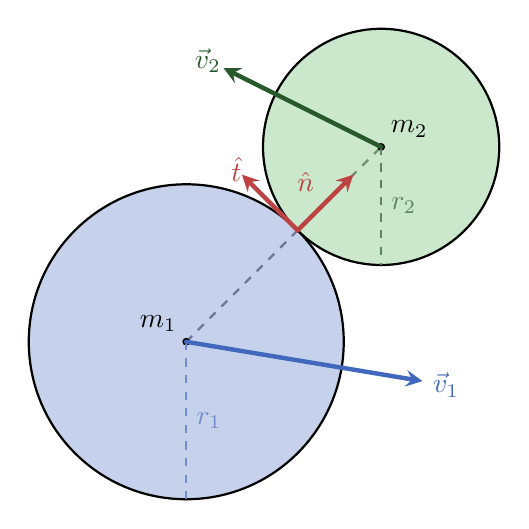
\begin{tikzpicture}
			\coordinate (xA) at (0, 0);
			\pgfmathsetmacro{\rA}{2}
			\pgfmathsetmacro{\rB}{1.5}
			\pgfmathsetmacro{\th}{45}
			\coordinate (xB) at ({(\rA+\rB)*cos(\th)},{(\rA+\rB)*sin(\th)});
			\coordinate (uAB) at ({\rA*cos(\th)},{\rA*sin(\th)});
			\draw[thick, dashed, black!50] (xA) -- (xB);

			\tikzset{
				sphere/.style={thick, fill=#1, fill opacity=0.3},
				radius/.style={thick, dashed, draw=#1},
			}
			\draw[sphere={xblue}]  (xA) circle (\rA);
			\draw[sphere={xgreen}] (xB) circle (\rB);
			\fill (xA) circle (0.05) node [above left]  {$m_{1}$};
			\fill (xB) circle (0.05) node [above right] {$m_{2}$};
			\draw[radius={xblue!75}] (xA) -- ++(0,-\rA) node [xblue!75, midway, right] {$r_{1}$};
			\draw[radius={xdarkgreen!75}] (xB) -- ++(0,-\rB) node [xdarkgreen!75, midway, right]  {$r_{2}$};

			\draw[vector={xblue}] (xA) -- ++(3,-0.5) node [pos=1.1] {$\vec{v}_{1}$};
			\draw[vector={xdarkgreen}] (xB) -- ++(-2,1.0) node [pos=1.1] {$\vec{v}_{2}$};

			\draw[vector={xred}] (uAB) -- ++({cos(\th)},{sin(\th)}) node [midway, above left] {$\hat{n}$};
			\draw[vector={xred}] (uAB) -- ++({cos(\th+90)},{sin(\th+90)}) node [pos=1.1] {$\hat{t}$};
		\end{tikzpicture}
	\end{center}
	\caption{Text text text}
	\label{fig:elastic_collision}
\end{figure}

Note that we did not define a coordinate system, nor the number of dimensions $d$ for the problem. The only restriction is that $d\geq2$.

Conservation of momentum means that the velocities of the spheres following the collision, $\vec{u}_{1},\vec{u}_2$, are related to their velocities before the collision by
\begin{equation}
	\begin{aligned}
		                 & m_{1}\vec{v}_{1} + m_{2}\vec{v}_{2} = m_{1}\vec{u}_{1} + m_{2}\vec{u}_{2}                   \\
		\Rightarrow\quad & m_{1}\left(\vec{v}_{1} - \vec{u}_{1}\right)  = m_{2}\left(\vec{u}_{2} - \vec{v}_{2}\right).
	\end{aligned}
	\label{eq:elastic_collision_coservation_of_momentum}
\end{equation}

Conservation of energy means that the velocities are also related by
\begin{equation}
	\begin{aligned}
		                 & \frac{1}{2}m_{1}\norm{\vec{v}_{1}}^{2} + \frac{1}{2}m_{2}\norm{\vec{v}_{2}}^{2} = \frac{1}{2}m_{1}\norm{\vec{u}_{1}}^{2} + \frac{1}{2}m_{2}\norm{\vec{u}_{2}}^{2} \\
		\Rightarrow\quad & m_{1}\left(\norm{\vec{v}_{1}}^{2} - \norm{\vec{u}_{1}}^{2}\right) = m_{2}\left(\norm{\vec{u}_{2}}^{2} - \norm{\vec{v}_{2}}^{2}\right).
	\end{aligned}
	\label{eq:elastic_collision_coservation_of_energy}
\end{equation}

However, the forces involved in the collision can not have a component in the $\hat{t}$ direction, and are limited to only point in the $\hat{n}$ direction. Therefore, we can reduce the problem to this direction only by projecting all velocities involved in the problem on $\hat{n}$, i.e. \autoref{eq:elastic_collision_coservation_of_momentum} becomes
\begin{equation}
	m_{1}\innerproduct{\vec{v}_{1}}{\hat{n}} + m_{2}\innerproduct{\vec{v}_{2}}{\hat{n}} = m_{1}\innerproduct{\vec{u}_{1}}{\hat{n}} + m_{2}\innerproduct{\vec{u}_{2}}{\hat{n}}.
	\label{eq:elastic_collision_coservation_of_momentum_projection}
\end{equation}

TEXT TEXT TEXT

\begin{equation}
	\begin{aligned}
		\vec{u}_{1} & = \vec{v}_{1} - \frac{2m_{2}}{m_{1}+m_{2}}\innerproduct{\vec{v}_{1}-\vec{v}_{2}}{\hat{n}}\hat{n}, \\
		\vec{u}_{2} & = \vec{v}_{2} + \frac{2m_{1}}{m_{1}+m_{2}}\innerproduct{\vec{v}_{1}-\vec{v}_{2}}{\hat{n}}\hat{n}.
	\end{aligned}
\end{equation}

To avoid reduntant calculations, we can factor out the common quantity of both velocities:
\begin{equation}
	K = \frac{2}{m_{1}+m_{2}}\innerproduct{\vec{v}_{1}-\vec{v}_{2}}{\hat{n}}\hat{n},
	\label{eq:elastic_collision_common_quantity}
\end{equation}
yielding
\begin{equation}
	\begin{aligned}
		\vec{u}_{1} & = \vec{v}_{1}-Km_{2}, \\
		\vec{u}_{2} & = \vec{v}_{2}+Km_{1}.
	\end{aligned}
	\label{eq:elastic_collision_final_equation}
\end{equation}

\subsection{Reducing collision test complexity}
% BBOX, Neighbor lists, etc.

% \section{Molecular Dynamics}

\makeatother

\end{document}
